\documentclass[12pt]{article}
\usepackage[a4paper, margin=1in]{geometry}
\usepackage{hyperref}
\usepackage{graphicx}
\graphicspath{{../figures/}}
\usepackage{float}
\usepackage{enumitem}
\usepackage{amsmath}

\title{Research Project - Mathematical Statistics}
\author{Katia Russo, Matteo Zabban}
\date{2024 / 2025}

\begin{document}

\maketitle
\tableofcontents

\newpage
\section{Introduction}
The admission process for graduate studies is a critical step in defining our future careers, as a consequence, it is filled with ambition as the volume of candidates competes for limited spots in prestigious programs. Among the factors that admission committees have to analyze, there are both quantitative (GRE, TOEFL, GPA, etc.) and qualitative metrics (recommendation letters, personal statements, etc.). As students deeply involved in this process, we were driven by curiosity to discover what sets successful candidates apart.

\vspace{10pt}
\indent Our study takes a systematic approach, delving into the aspects of admissions and carefully analyzing the contributions of each factor. This project, therefore, holds the potential to provide key insights that may guide future applicants in optimizing their profiles for success. The competitive landscape of higher education, marked by an ever-growing pool of talented individuals, makes this endeavor very significant.


\section{Dataset}
The dataset used in this analysis, titled \textit{Graduate Admission 2}, was sourced from Kaggle and is distributed under the CC0 public license, meaning it is in the public domain. For transparency and reproducibility, the link to the dataset will be included in the bibliography section of this report \hyperref[b]{\scriptsize {(Bibliography)}}.

\vspace{10pt}
\indent This dataset is inspired by the UCLA Graduate Dataset, widely known in academic circles for admissions-related studies. It is important to note that the test scores and GPA in this dataset are presented in their older formats, which differ from the formats currently in use.

\vspace{10pt}
\indent The dataset consists of 500 observations, each corresponding to an individual applicant to a graduate program. The observations provide a structured representation of applicants’ profiles, including quantitative metrics and a target variable indicating the likelihood of admission. Specifically, the dataset includes the following variables:

\begin{enumerate}[noitemsep]
    \item \textbf{Serial.No.}: Identification number of application.
    \item \textbf{GRE.Score}: Applicant’s Graduate Record Examination score [0, 340].
	\item \textbf{TOEFL.Score}: Applicant’s Test of English as a Foreign Language score [0, 120].
	\item \textbf{University.Rating}: A ranking of the university from which the applicant graduated [1, 5].
	\item \textbf{SOP}: Applicant’s Statement of Purpose [1, 5].
	\item \textbf{LOR}: Applicant’s Letters of Recommendation [1, 5].
	\item \textbf{CGPA}: Applicant’s undergraduate Grade Point Average [0, 10].
	\item \textbf{Research}: A binary variable indicating whether the applicant has prior research experience (1 for yes, 0 for no).
	\item \textbf{Chance.of.Admit}: A continuous variable ranging from 0 to 1, representing the predicted probability of admission to the program.
\end{enumerate}

\subsection{Data Cleaning}
Before moving on to data analysis, we performed what is known as \textit{Data Cleaning}. These steps were essential to ensure that the data was ready for exploration, reducing the risk of encountering errors later on. The first column, \textit{Serial.No.}, was removed as it was not useful for our study; it served only as an identifier and did not provide any predictive value. The dataset was then checked for any missing values, and since none were found, we were able to proceed.

\vspace{10pt}
\indent Boxplots of the continuous variables were used to detect outliers, as these kinds of extreme values can skew results and impact the accuracy of the model. Fortunately, no significant outliers were identified. Next, we reviewed the data for its format: histograms of continuous variables showed that they were on meaningful scales, and the binary variable, \textit{Research}, was encoded using only 0/1 as unique values, making it suitable for our study without further adjustments. These steps ensured that our dataset was clean, consistent, and ready for statistical modeling. \hyperref[cleaning]{\scriptsize {(Appendix A.1)}}

\subsection{Data Visualization}
Data visualization plays a vital role in understanding relationships and distributions within the dataset, offering valuable insights that guide further analysis. To explore the connections between the target variable, \textit{Chance.of.Admit}, and each predictor, scatter-plots were created for all combinations \hyperref[cleaning]{\scriptsize {(Appendix A.1)}}, the following are the most significant ones. 


\begin{figure}[H]
    \centering
    \begin{minipage}{0.3\textwidth}
        \centering
        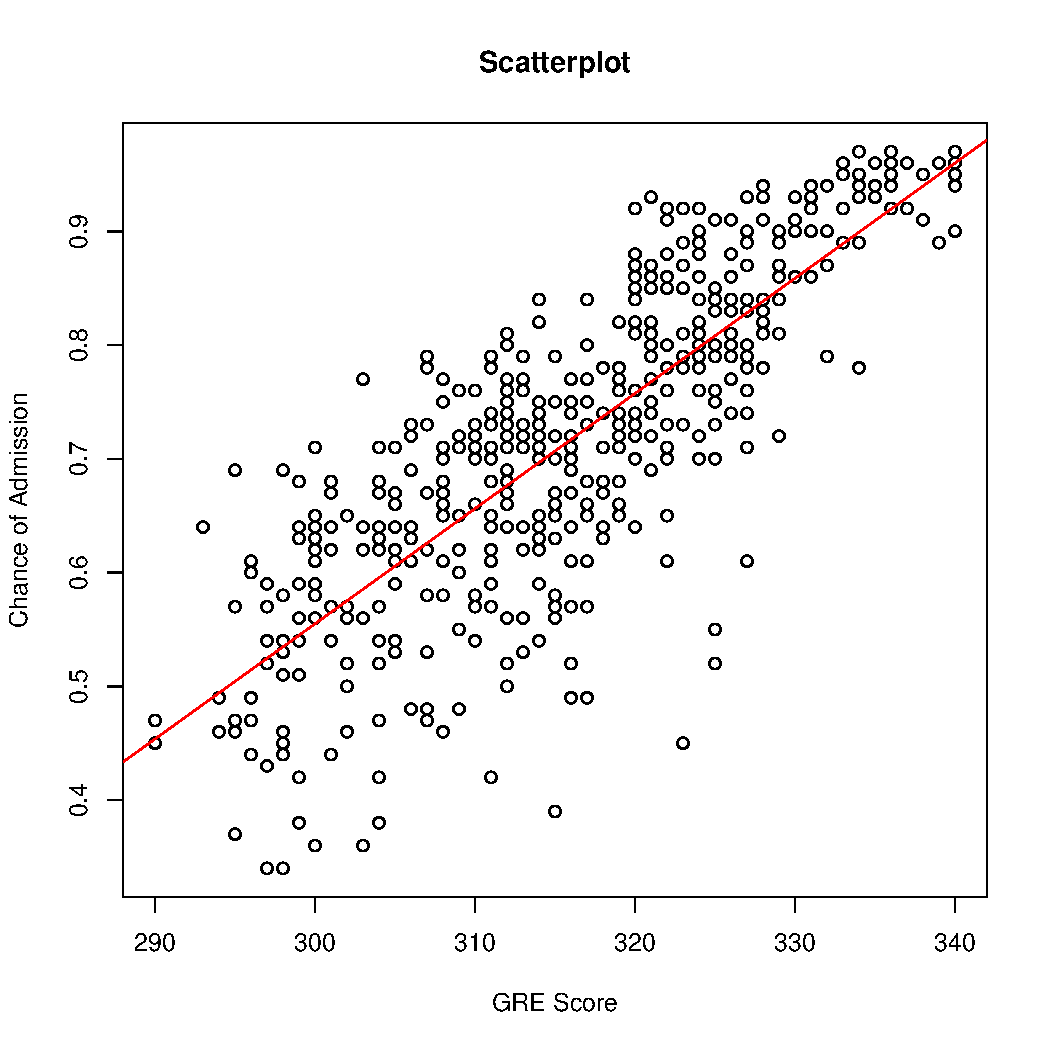
\includegraphics[width=\textwidth]{scatterplotGRE.pdf}
    \end{minipage}
    \begin{minipage}{0.3\textwidth}
        \centering
        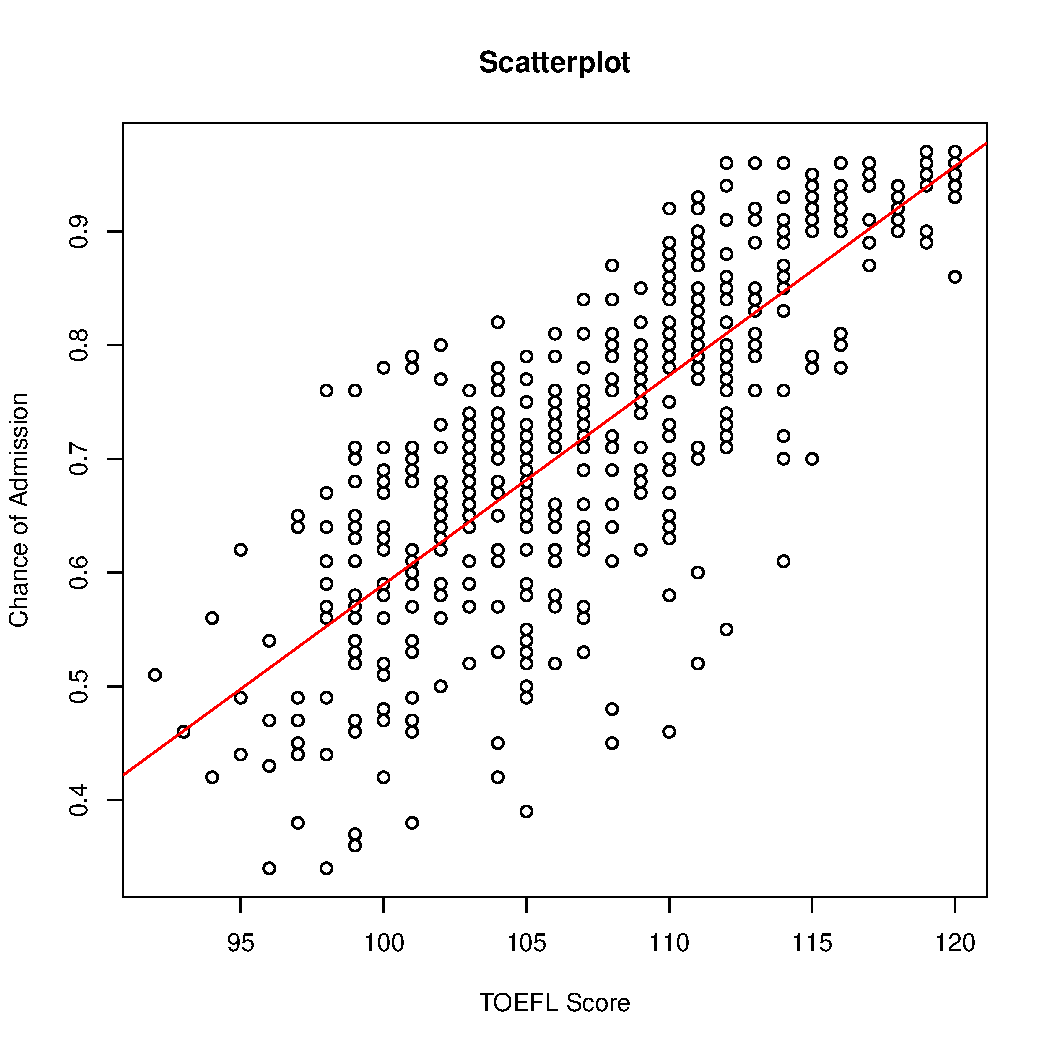
\includegraphics[width=\textwidth]{scatterplotTOEFL.pdf}
    \end{minipage}
    \begin{minipage}{0.3\textwidth}
        \centering
        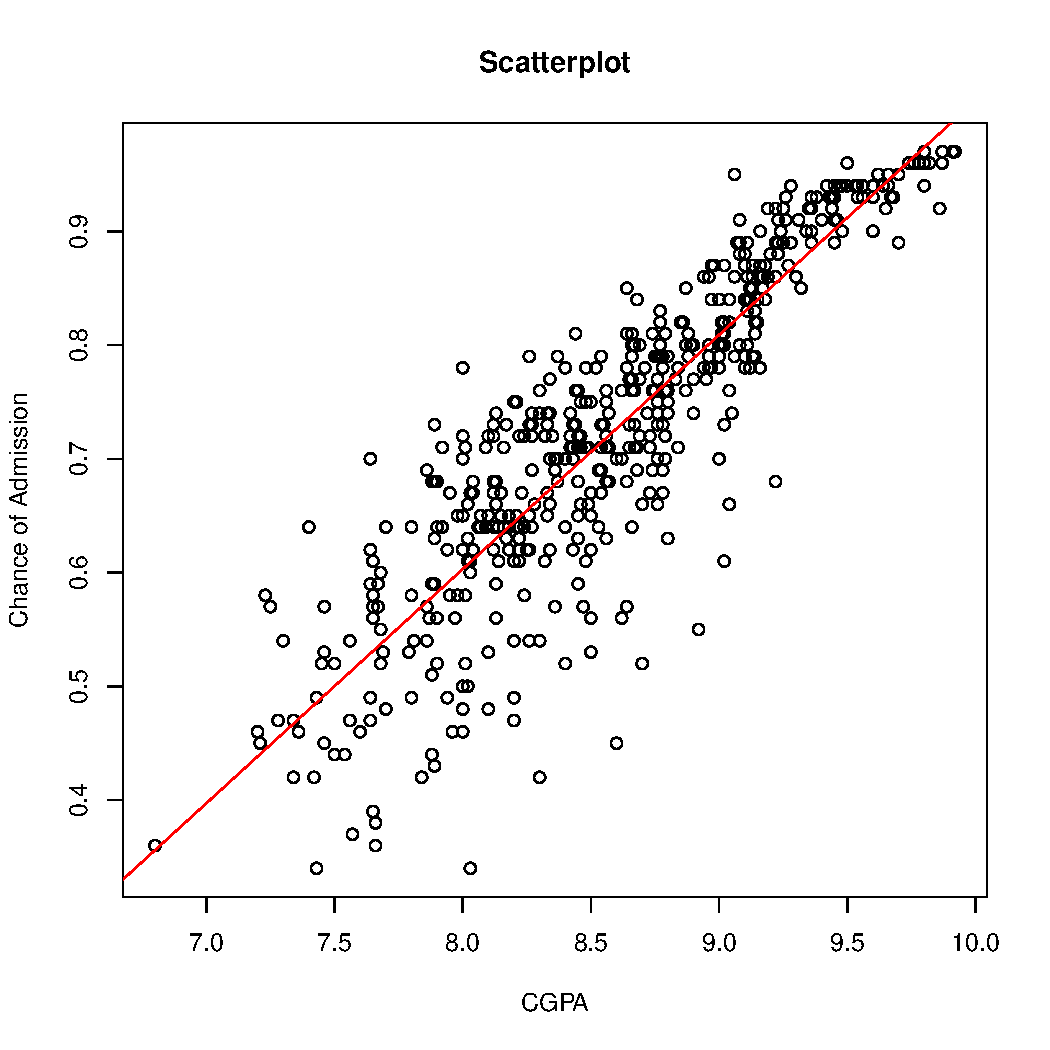
\includegraphics[width=\textwidth]{scatterplotCGPA.pdf}
    \end{minipage}
\end{figure}



\section{Regression Model}
The objective of this section is to estimate the relationships between the predictors and the target variable \textit{Chance.of.Admit} using a multiple linear regression model. This approach allows us to quantify the impact of each predictor on the likelihood of admission while accounting for the effects of other variables.
A multiple linear regression model was fitted to the data using the equation:
\[
Y_i = \beta_0 + \beta_1 X_{1i} + \beta_2 X_{2i} + ... + \beta_p X_{pi} + e_i \quad \text{with } i = 1, ..., n \quad n = 500
\]
where  \(Y_i\)  represents the \textit{Chance.of.Admit} for the \(i\)-th observation,  \(X_{1i}, X_{2i}, \ldots, X_{pi}\)  are the predictors,  \(\beta_j\)  are the regression coefficients representing the effect of each predictor, and  \(\epsilon_i\)  is the random error term for the \(i\)-th observation.

\subsection{Validity assumptions}
Before interpreting the results, we run diagnostic checks to validate the model’s assumptions and ensure its reliability.
The QQ plot of the residuals indicates that they are approximately normally distributed, even though there are minor deviations at the tails. This suggests that normality is mostly but not entirely satisfied, as showed by the Shapiro-Wilk test. The histogram of residuals further supports this observation, showing a roughly symmetric bell-shaped distribution centered around zero.

\vspace{10pt}
\indent The residuals versus fitted values plot shows no clear pattern, which suggests that the assumption of homoscedasticity is almost satisfied, as the residual variance doesn't appear constant across all fitted values. However, there is some slight non-linearity observable in the residuals, indicating that the assumption of linearity between predictors and the target variable is only partially met. In addition, multicollinearity was examined with a correlation matrix to ensure that no predictor was excessively correlated with another. \hyperref[SW]{\scriptsize {(Appendix A.2)}}.

\begin{figure}[H]
    \centering
    \begin{minipage}{0.3\textwidth}
        \centering
        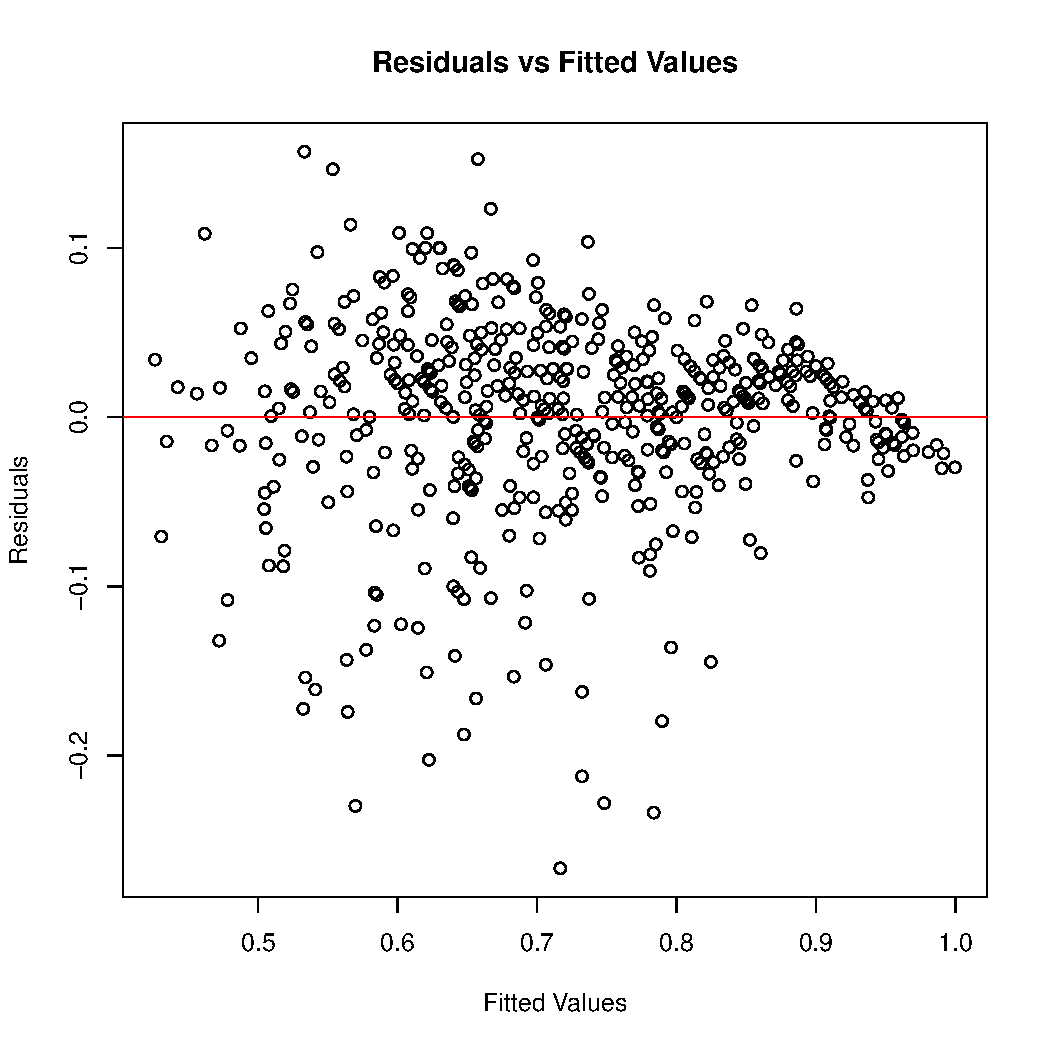
\includegraphics[width=\textwidth]{RFV.pdf}
    \end{minipage}
    \begin{minipage}{0.3\textwidth}
        \centering
        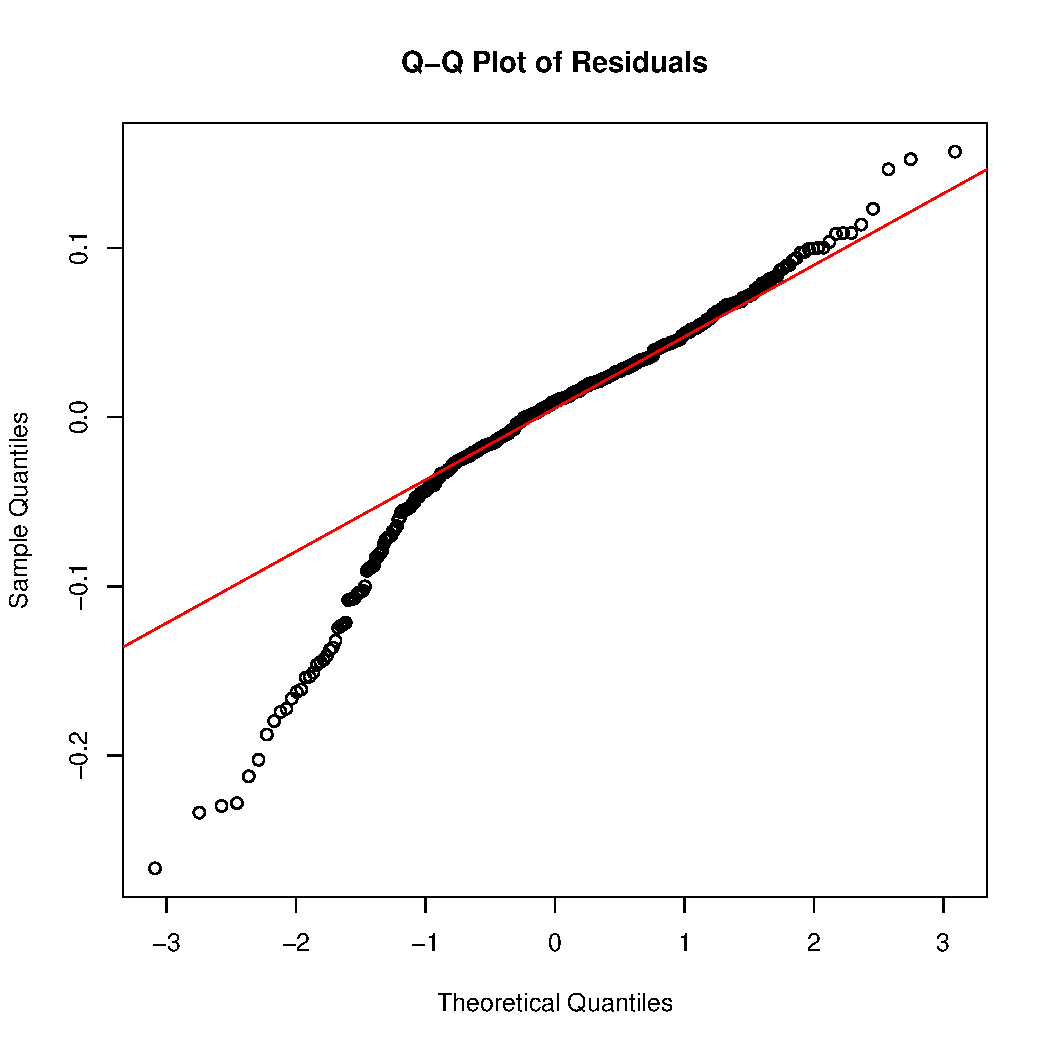
\includegraphics[width=\textwidth]{QQR.pdf}
    \end{minipage}
    \begin{minipage}{0.3\textwidth}
        \centering
        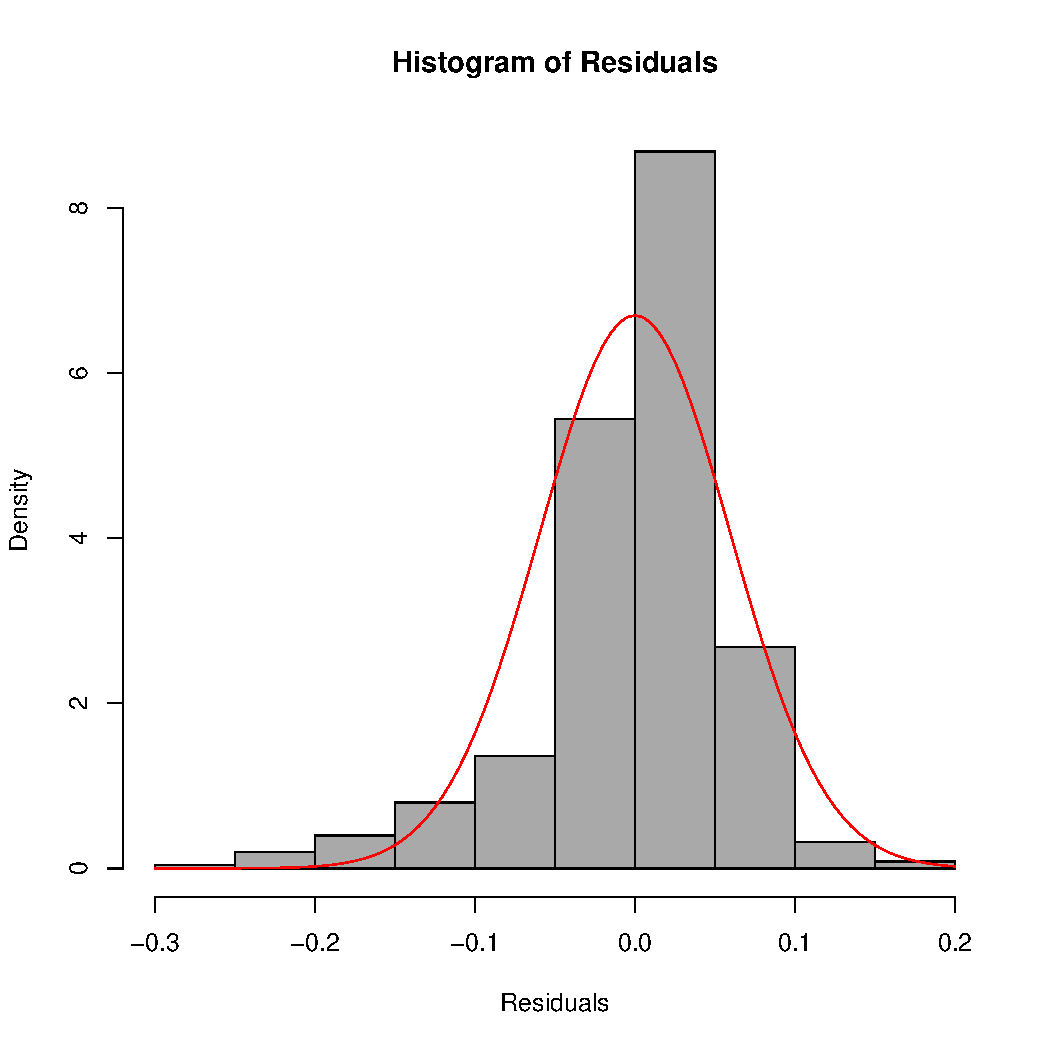
\includegraphics[width=\textwidth]{HR.pdf}
    \end{minipage}
\end{figure}

\subsection{Interaction Effects}
Interaction effects are crucial in regression analysis as they capture interdependencies between predictors and the response variable. To explore the potential interaction between \textit{Research} and \textit{University.Rating}, an interaction plot was first created to visualize their combined effect on \textit{Chance.of.Admit}. The plot suggested a dependency, prompting us to include an interaction term in the model for further analysis.

\vspace{10pt}
\indent An \textbf{ANOVA} test comparing the baseline model and the interaction model confirmed a significant improvement ( \(F\) = 5.1605 ,  \(p\) = 0.02354 ), rejecting the null hypothesis that the interaction term does not enhance the model. While the improvement in adjusted  \(R^2\)  was marginal, increasing from 0.8194 to 0.8209, and the reduction in residual standard error was minimal, the interaction term added interpretive depth. The coefficient for the interaction term ( \(\beta\) = 0.0123, \(p\) = 0.02354 ) indicates that the relationship between \textit{University.Rating} and \textit{Chance.of.Admit} is influenced by \textit{Research}. \hyperref[SW]{\scriptsize {(Appendix A.2)}} Although the improvement in model performance was slight, the interaction term provides valuable insights into the interplay between predictors. Applicants with prior research experience from top-rated universities may have an advantage, as admissions committees often correlate such profiles with stronger academic and professional preparation.


\begin{figure}[H]
    \begin{minipage}{0.3\textwidth}
        \centering
        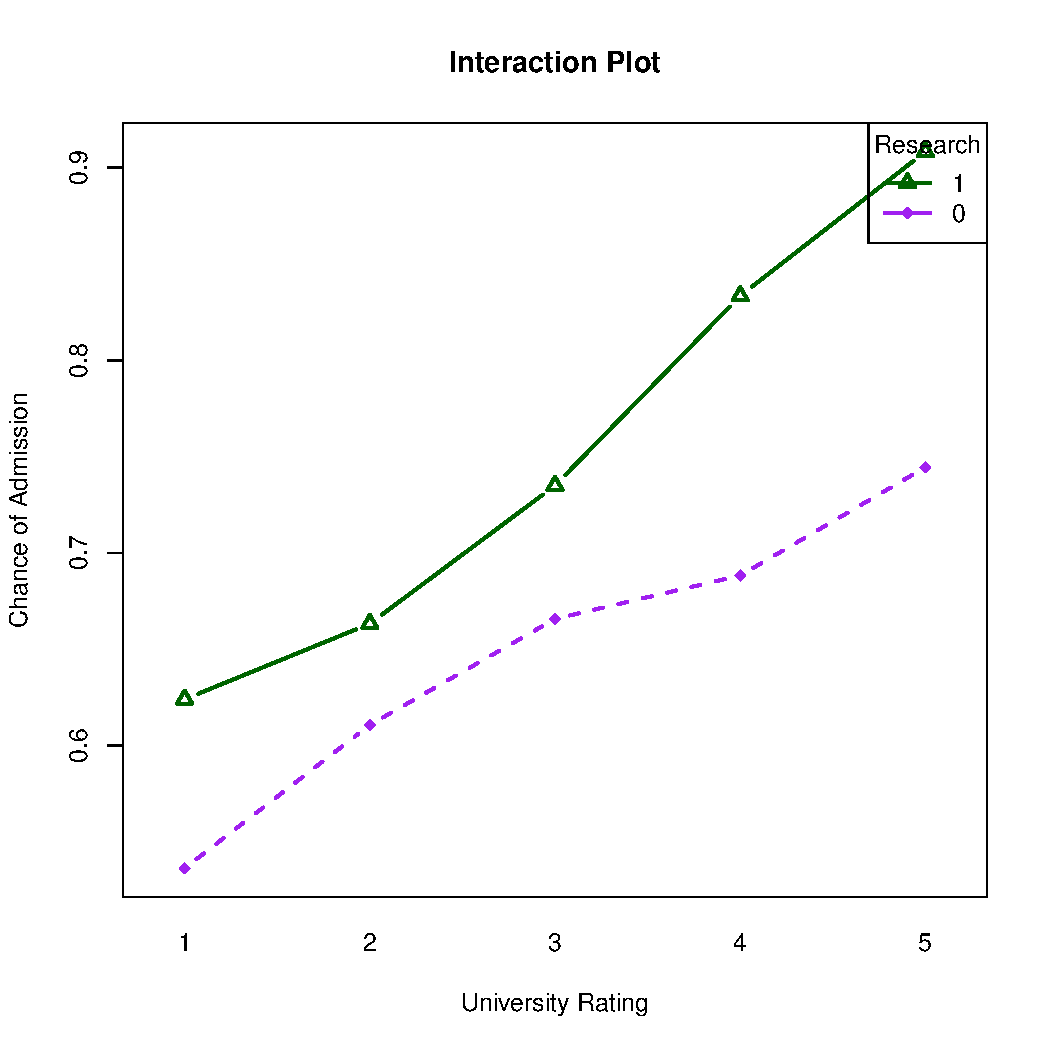
\includegraphics[width=\textwidth]{IP.pdf} % Adjust the width to make it smaller or larger
    \end{minipage}
    \hspace{0.5cm} % Add horizontal space between the images
    \begin{minipage}{0.3\textwidth}
        \centering
        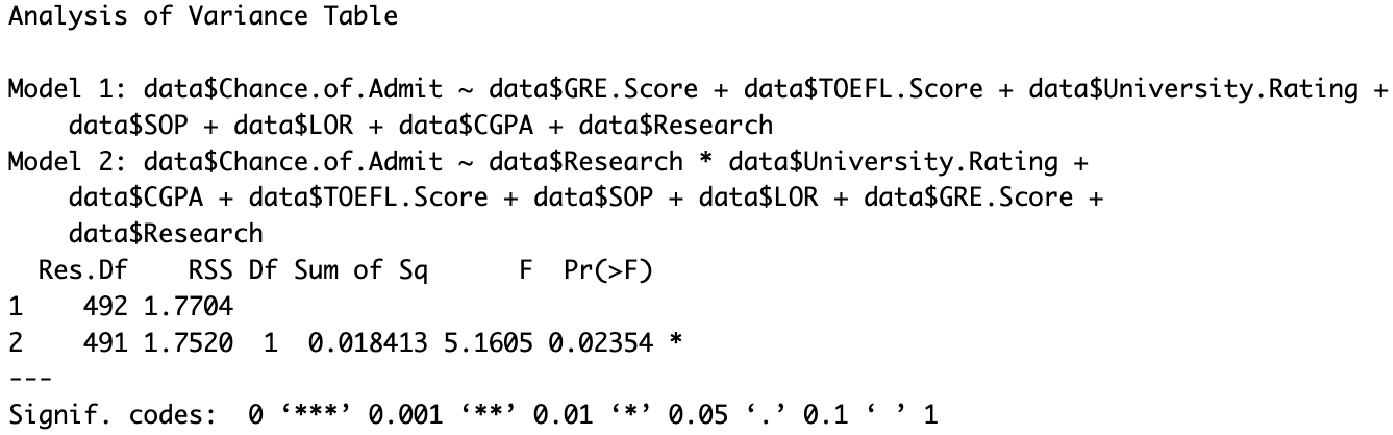
\includegraphics[width=2.3\textwidth]{anova.pdf} % Adjust the width to make it larger
    \end{minipage}
\end{figure}

\section{Model Selection}
\subsection{Step-down method}
To improve the regression model and ensure it balances simplicity and predictive accuracy, we decided to apply a step-down method based on backward elimination. Starting with the full model, which includes all main effects and the significant interaction term, this approach will iteratively tests the null hypothesis  \(H_0: \theta_i = 0\)  for each parameter. If the \textit{p-value} for a parameter exceeds the chosen significance threshold (0.05), the parameter is removed, and the model is refitted with the remaining parameters. This process continues, eliminating one parameter at a time, until all remaining parameters are statistically significant.

\vspace{10pt}
\indent The parameter \textit{SOP} was removed due to its lack of statistical significance (p = 0.64) in the full model.
In order to evaluate model performance we conducted a comparison between the full and the refined model. The full model had an adjusted \(R^2\) of 0.8209, while the refined model achieved a slightly improved adjusted \(R^2\) of 0.8212, indicating that the removal of non-significant terms did not compromise explanatory power. In terms of model fit criteria, the refined model outperformed the full model with a lower \textbf{AIC} and \textbf{BIC}, confirming that the refined model achieves a better balance between fit and simplicity. The residual standard error for the refined model was 0.05969, compared to 0.05973 for the full model, indicating a marginal improvement in residual variance. We then run a diagnostic over the refined model to check the validity of the assumptions.
 \hyperref[MS]{\scriptsize {(Appendix A.3)}}

\begin{figure}[H]
    \centering
    \begin{minipage}{0.3\textwidth}
        \centering
        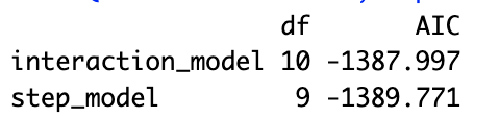
\includegraphics[width=1\textwidth]{AIC.pdf} 
    \end{minipage}
    \hspace{2cm}
    \begin{minipage}{0.3\textwidth}
        \centering
        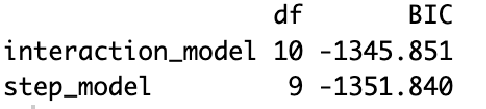
\includegraphics[width=1\textwidth]{BIC.pdf}
    \end{minipage}
\end{figure}

\subsection{Cross Validation}
The objective of this analysis was to validate the refined regression model and assess its predictive power using k-fold cross-validation. We selected 10-fold cross-validation as a balance between bias and variance in model evaluation. Using fewer folds, such as 5, might introduce higher variance in the results because each test set would contain fewer observations. Conversely, increasing the number of folds (e.g., 20-fold) could reduce variance but significantly increase computational cost without substantial gains in model performance. The 10-fold approach offers an optimal trade-off between computational efficiency and the robustness of results.
The model was trained on 9 folds and tested on the remaining one, with this process repeated across all folds, ensuring that every observation is used for both training and testing. The results showed an average  \(R^2\)  of 0.820, indicating the model explains a significant portion of the variance in \textit{Chance.of.Admit}, with an RMSE of 0.060. The low standard deviations for  \(R^2 \)  and RMSE confirm the model’s predictive power.

\begin{center}
    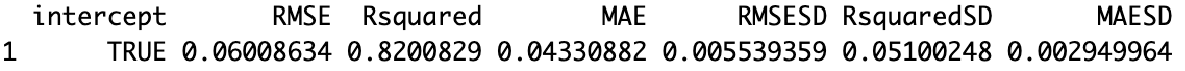
\includegraphics[width=0.8\textwidth]{KFCV.pdf}
\end{center}

\section{Limitations and conclusions}
This project provided insights into which factors mostly influence the chance of admission to graduate programs, while also validating a predictive model. From this analysis, it emerged that the most significant predictors are academic credentials, such as GPA, GRE and TOEFL, suggesting that candidates should prioritize excelling academically. Nevertheless research experience, combined with university rating, remains significant. The final model, validated through 10-fold cross-validation, exhibited strong predictive power, explaining over 82\% of the variance in chance of admission with minimal prediction errors, confirming its reliability and generalizability.

\vspace{10pt}
\indent The analysis encountered several limitations that may have influenced the results. Although the dataset contained 500 observations and captured academic and personal variables, it may still be too small to capture more complex relationships. Moreover, the multicollinearity between variables, such as \textit{GRE.Score} and \textit{TOEFL.scores}, may have introduced bias in the estimates of the coefficients. The assumptions of linear regression were partially met; although the residual plots showed approximate linearity and homoscedasticity, the Shapiro-Wilk test revealed a deviation from normality that may cause issues with the reliability of confidence intervals and hypothesis tests, particularly in small datasets.

\vspace{10pt}
\indent These results underline the importance of academic performance in shaping admissions outcomes, while also highlighting opportunities for further research. In order to improve the accuracy of this predictive model, one could adopt different strategies such as non-parametric bootstrapping to generate robust confidence intervals and p-values, data transformations (e.g., log) or non-linear models to better capture complex relationships and address residual non-normality. Additionally, investigating the practical significance of interaction effects and employing more diverse validation techniques would provide a deeper understanding of the factors driving admission outcomes. This study serves as a rigorous foundation for future analyses, combining theoretical and empirical rigor to inform the graduate admissions process.


\newpage
\appendix

\section{Appendix : Supplementary Material}
\vspace{1cm}
\subsection{Data Set}
\label{cleaning}
\vspace{10pt}
\begin{itemize}
    \item Boxplots for checking outliers
        \begin{figure}[H]
        \centering
            \begin{minipage}{0.3\textwidth}
                \centering
                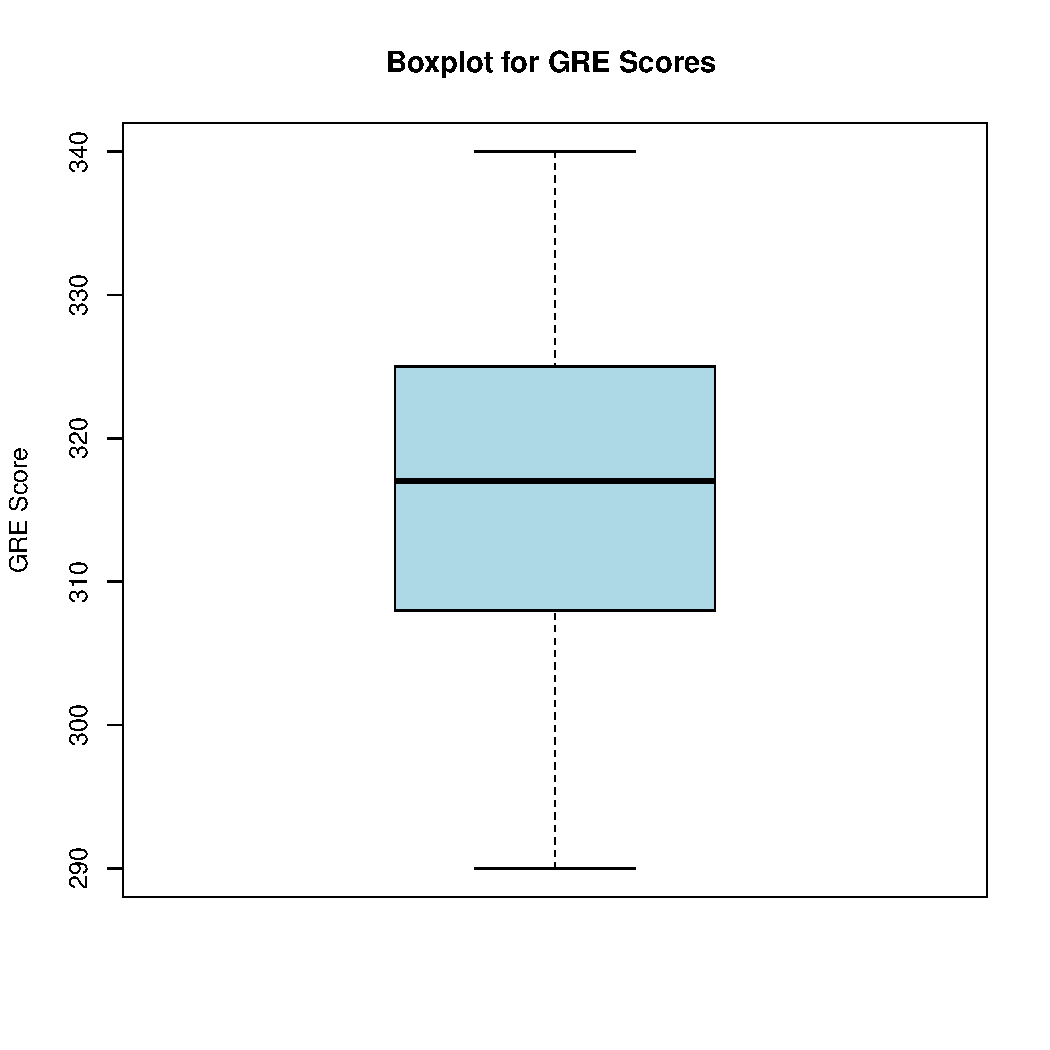
\includegraphics[width=\textwidth]{boxplotGRE.pdf}
            \end{minipage}
            \begin{minipage}{0.3\textwidth}
                \centering
                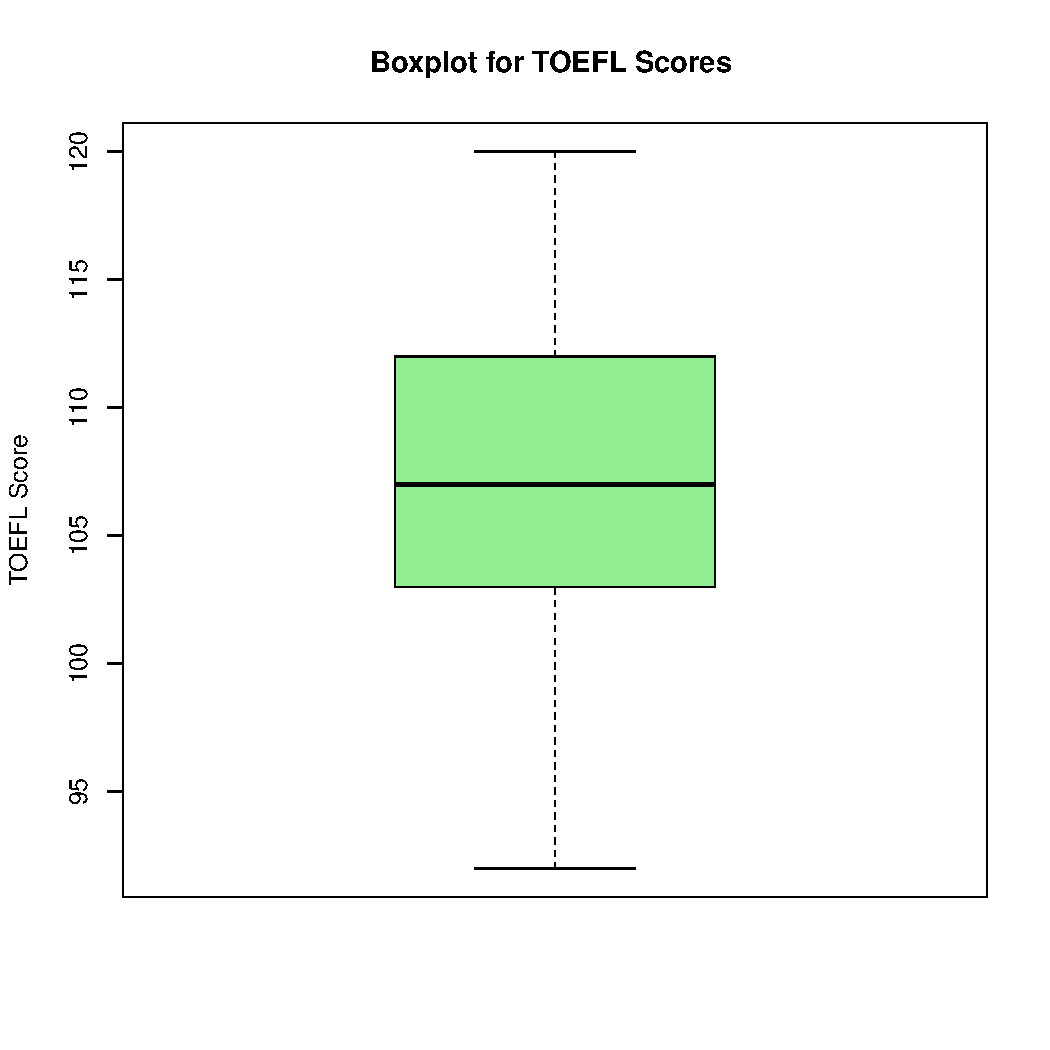
\includegraphics[width=\textwidth]{boxplotTOEFL.pdf}
            \end{minipage}
            \begin{minipage}{0.3\textwidth}
                \centering
                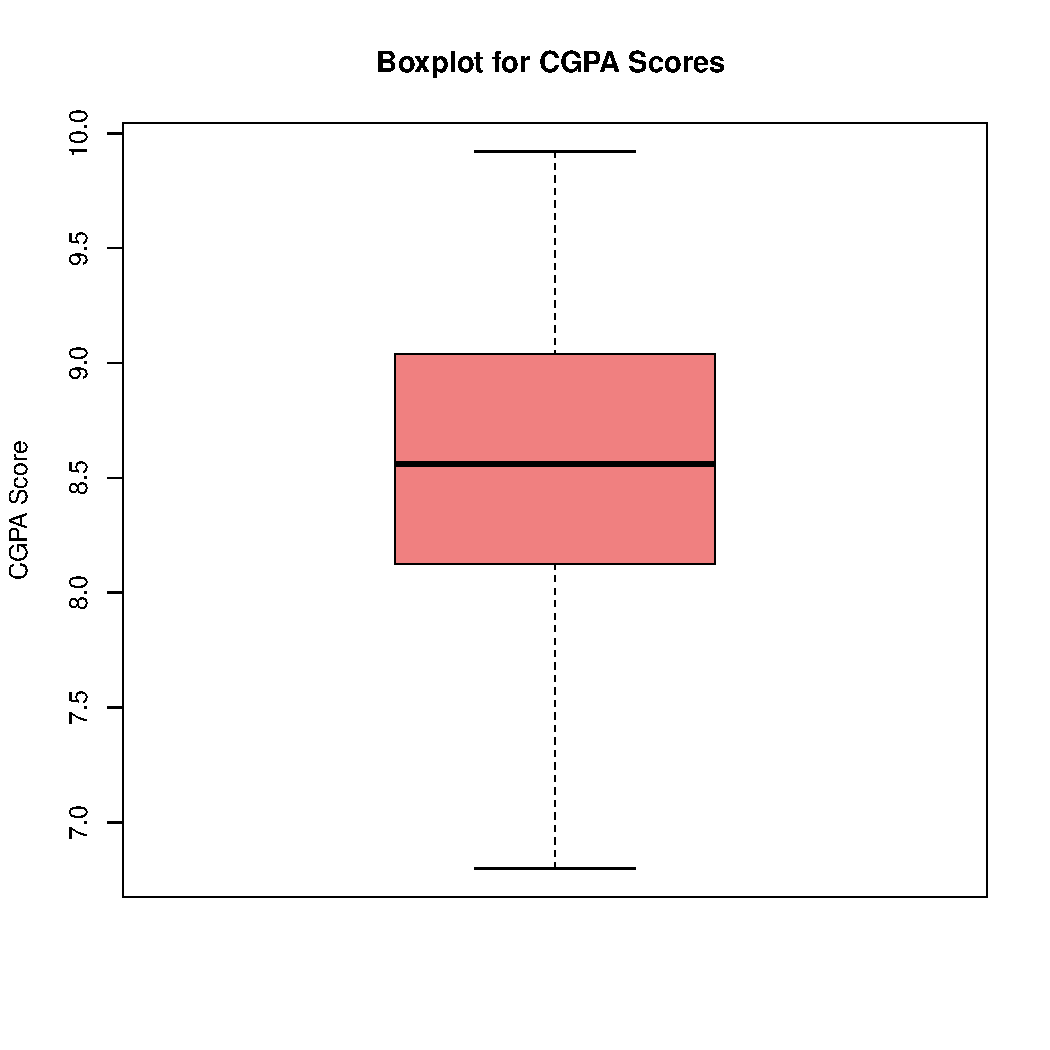
\includegraphics[width=\textwidth]{boxplotCGPA.pdf}
            \end{minipage}
        \end{figure}
    \item Histograms for continuous variables scale and distribution
        \begin{figure}[H]
            \centering
            \begin{minipage}{0.3\textwidth}
                \centering
                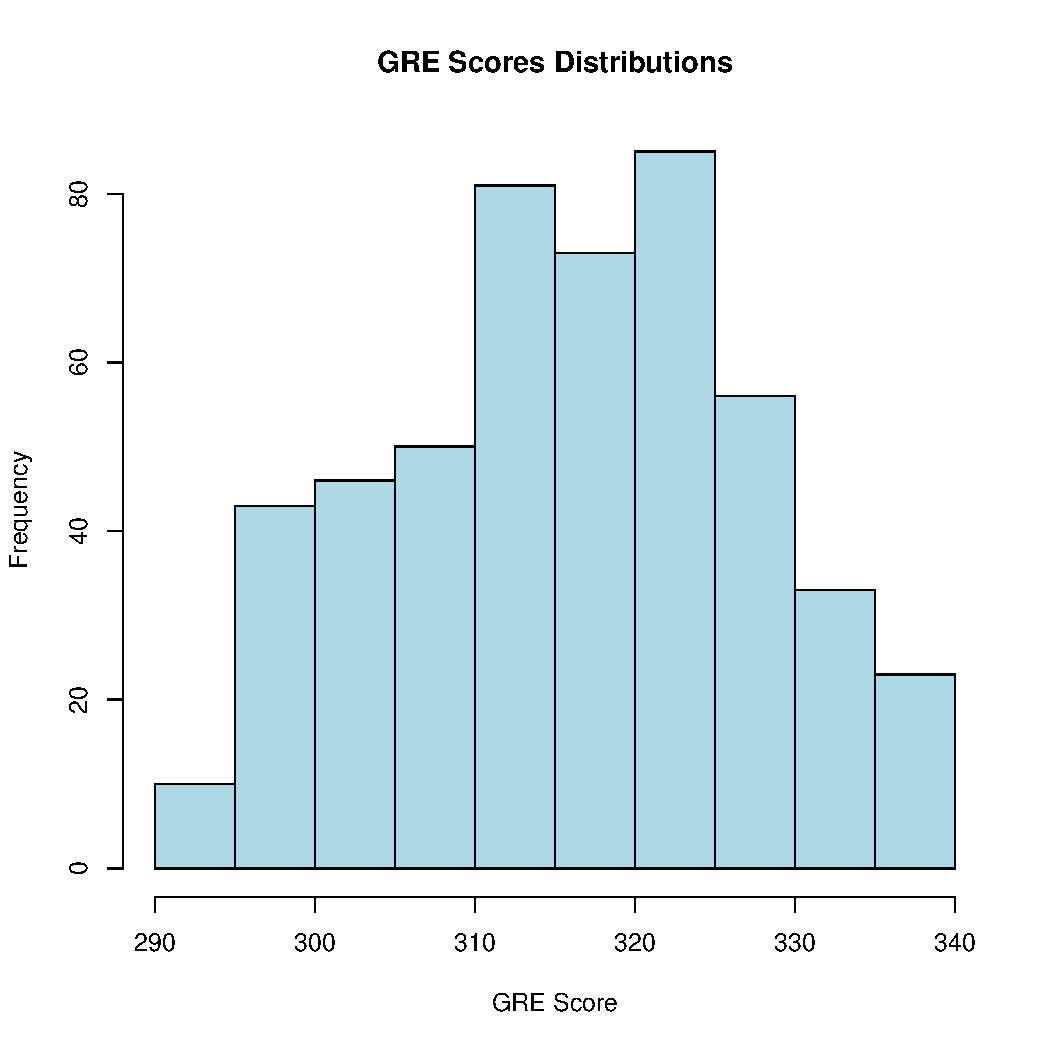
\includegraphics[width=\textwidth]{histogramGRE.pdf}
            \end{minipage}
            \begin{minipage}{0.3\textwidth}
                \centering
                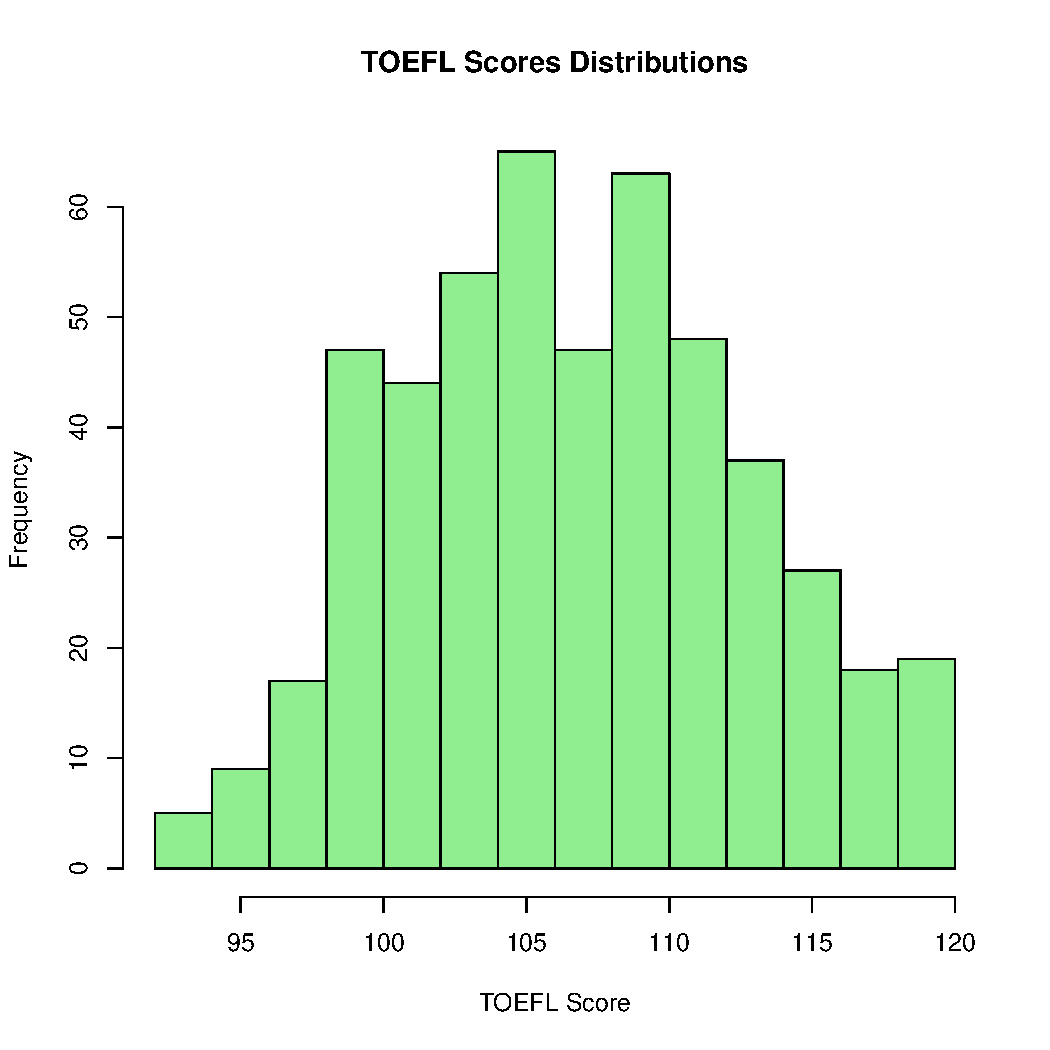
\includegraphics[width=\textwidth]{histogramTOEFL.pdf}
            \end{minipage}
            \begin{minipage}{0.3\textwidth}
                \centering
                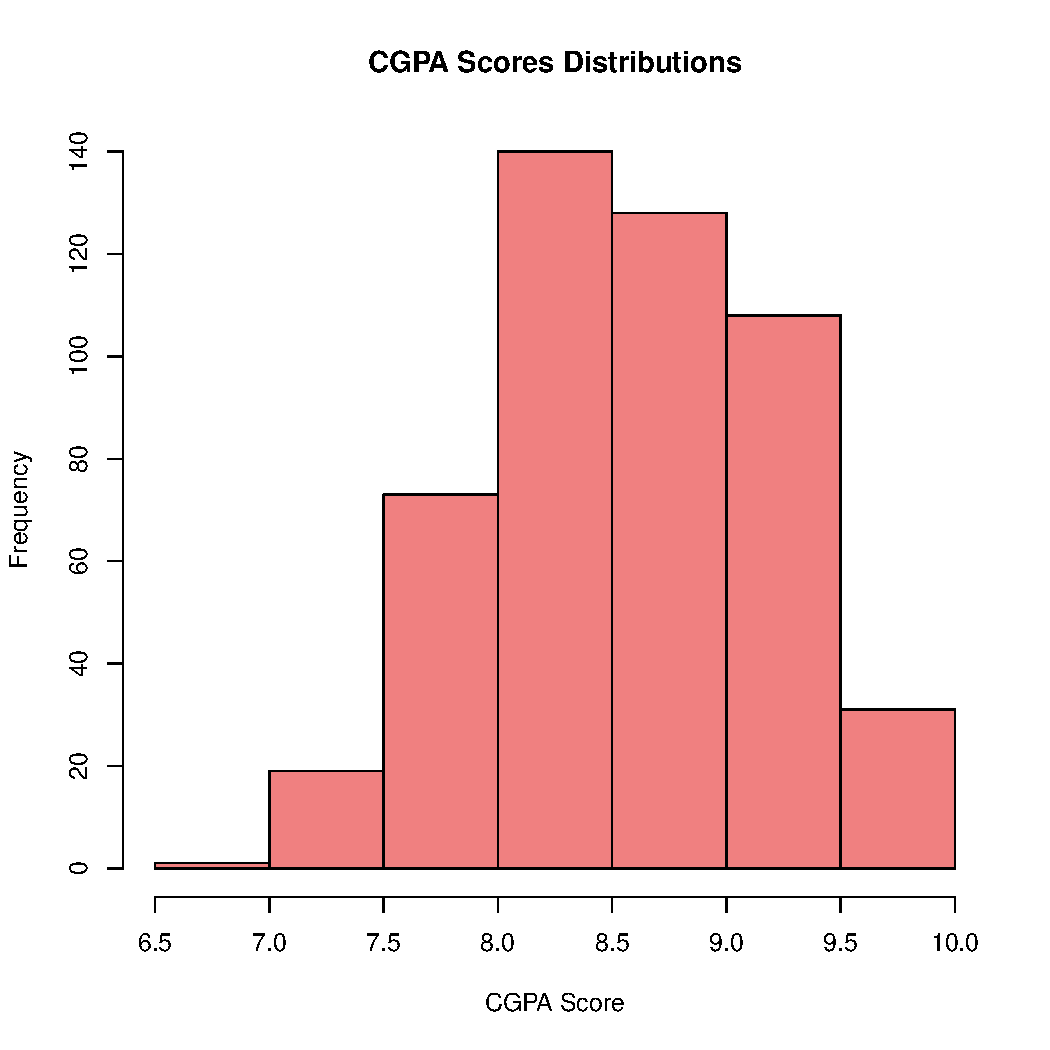
\includegraphics[width=\textwidth]{histogramCGPA.pdf}
            \end{minipage}
        \end{figure}
    \item First summary of the data
        \begin{figure} [H]
            \hspace{0.6cm}
            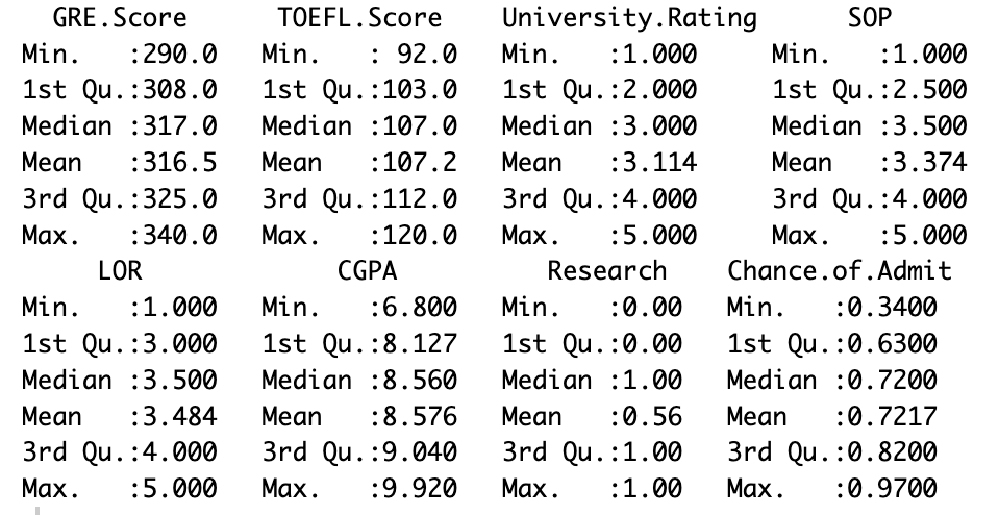
\includegraphics[width=0.8\linewidth]{dataS.pdf}
        \end{figure}
    \item Scatter plots
        \begin{figure}[H]
            \centering
            \begin{minipage}{0.3\textwidth}
                \centering
                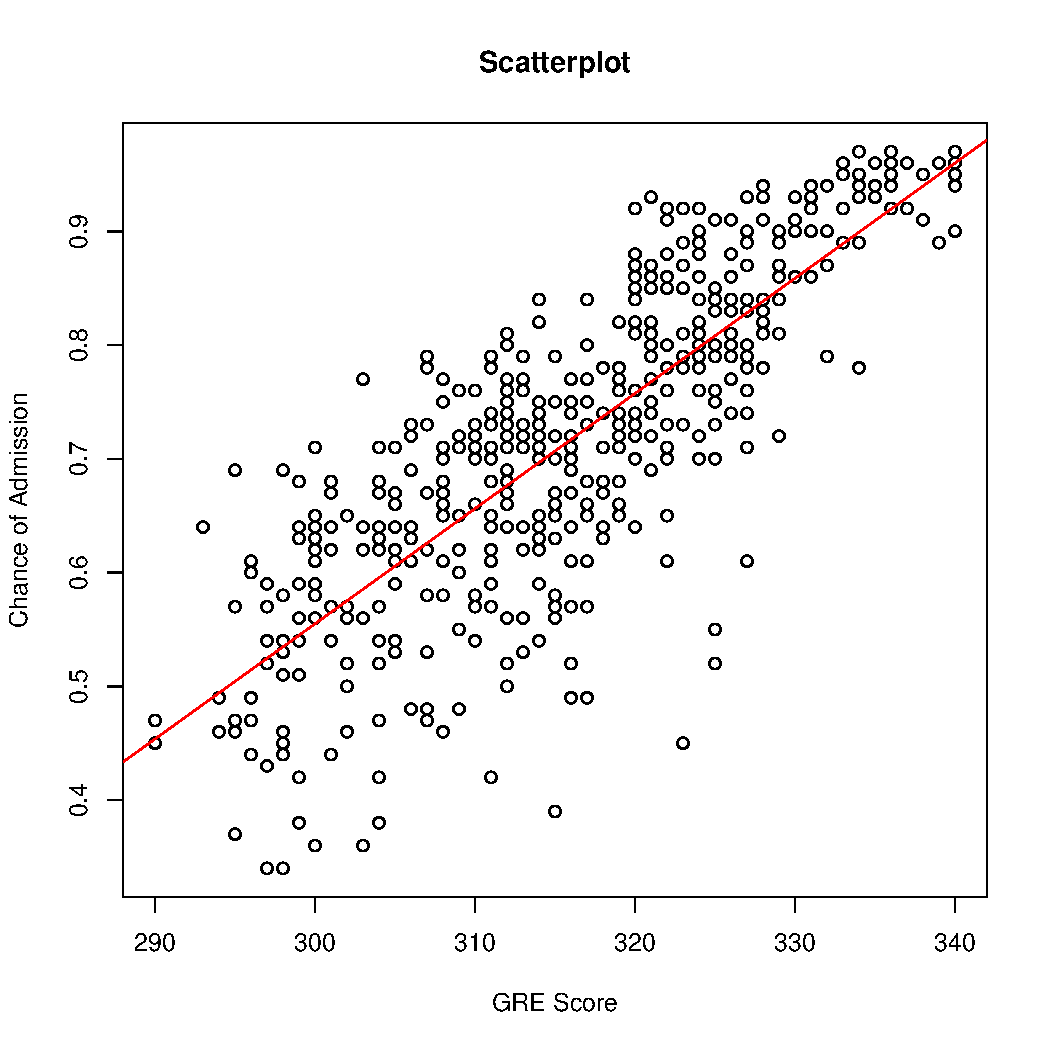
\includegraphics[width=\textwidth]{scatterplotGRE.pdf}
            \end{minipage}
            \begin{minipage}{0.3\textwidth}
                \centering
                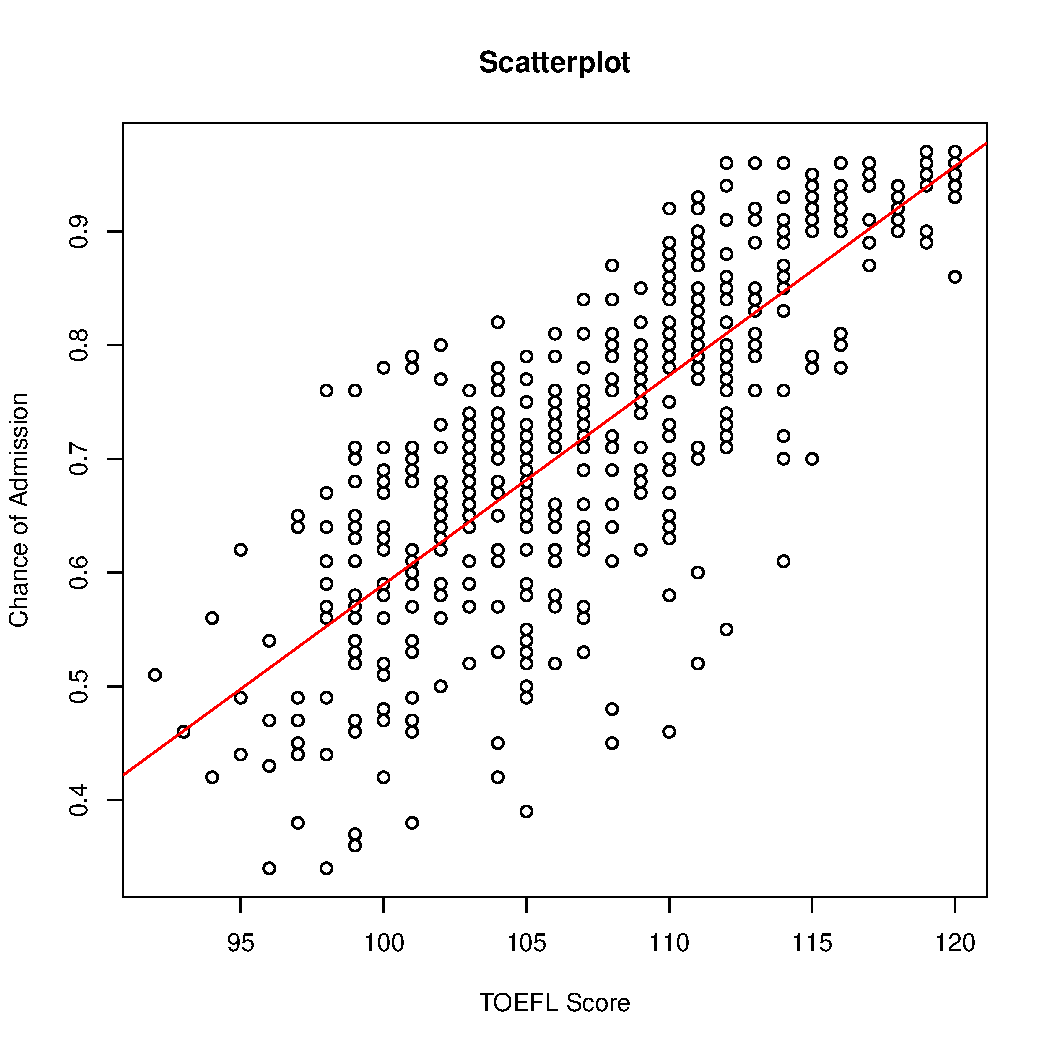
\includegraphics[width=\textwidth]{scatterplotTOEFL.pdf}
            \end{minipage}
            \begin{minipage}{0.3\textwidth}
                \centering
                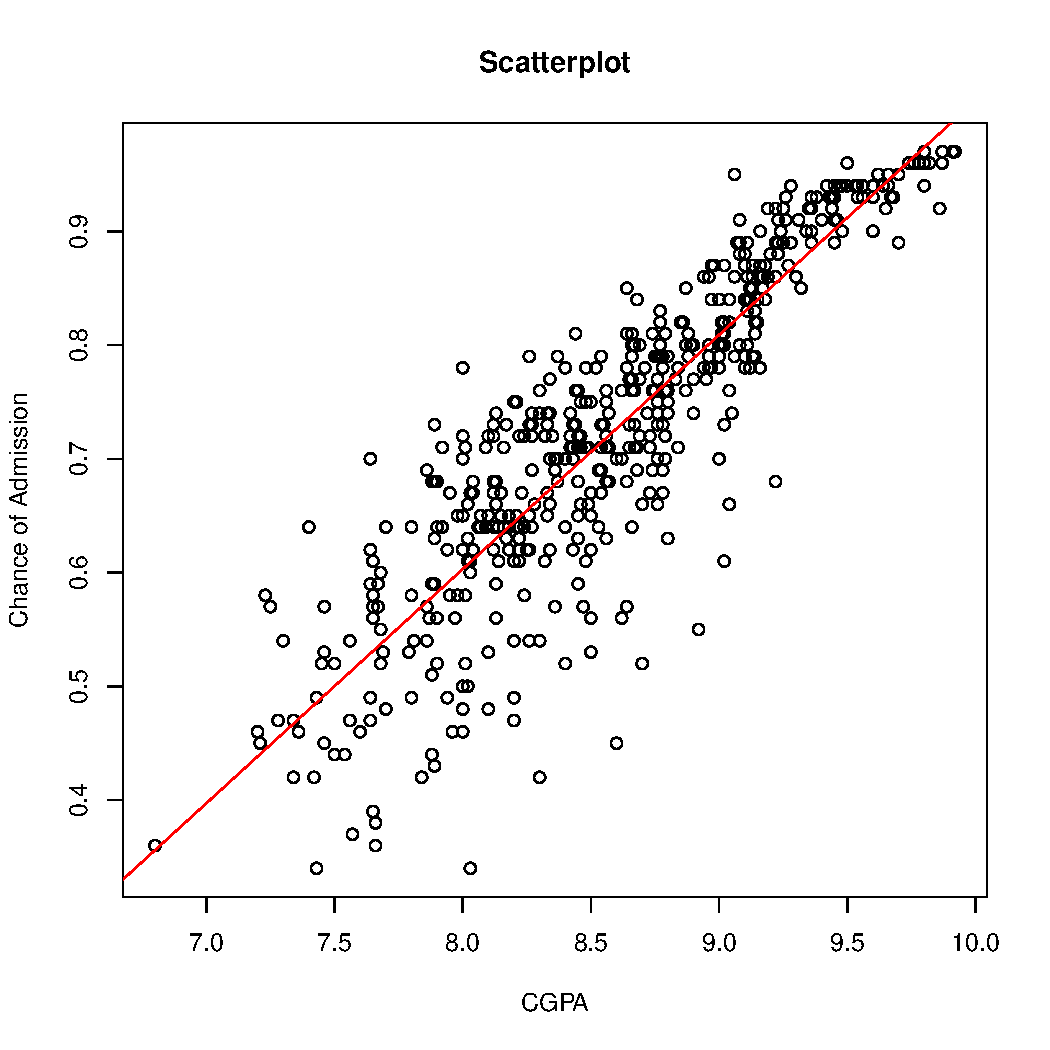
\includegraphics[width=\textwidth]{scatterplotCGPA.pdf}
            \end{minipage}
        \end{figure}
        \vspace{-1cm}
        \begin{figure}[H]
            \centering
            \begin{minipage}{0.3\textwidth}
                \centering
                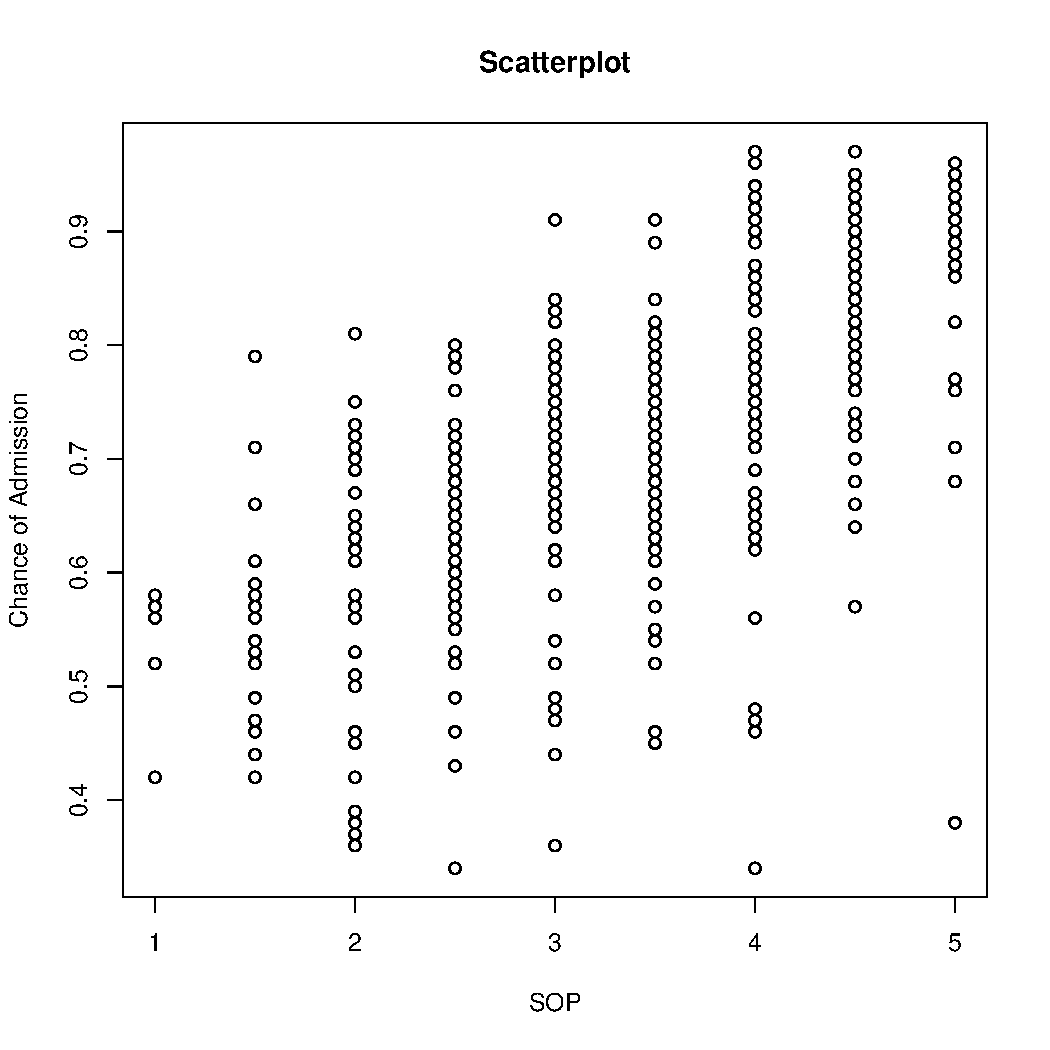
\includegraphics[width=\textwidth]{scatterplotSOP.pdf}
            \end{minipage}
            \begin{minipage}{0.3\textwidth}
                \centering
                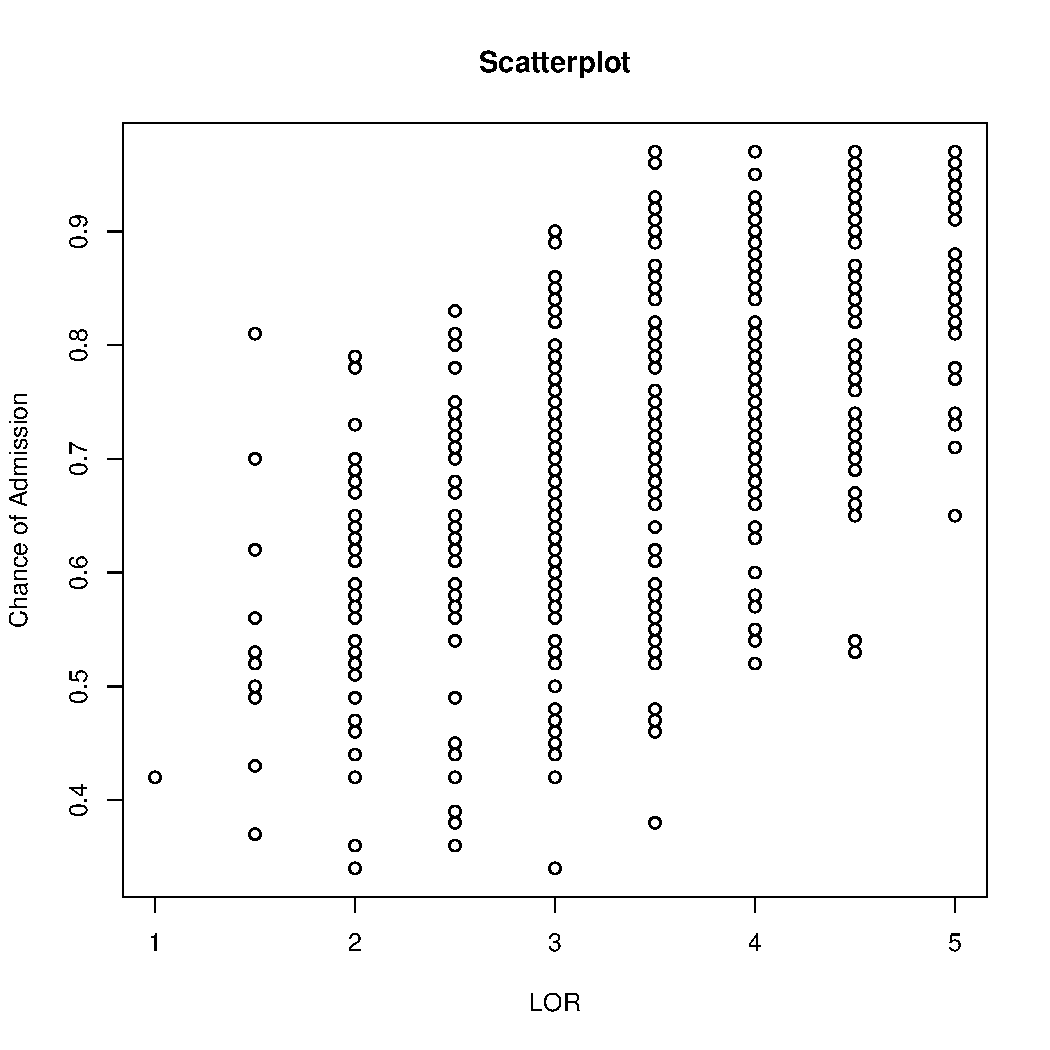
\includegraphics[width=\textwidth]{scatterplotLOR.pdf}
            \end{minipage}
            \begin{minipage}{0.3\textwidth}
                \centering
                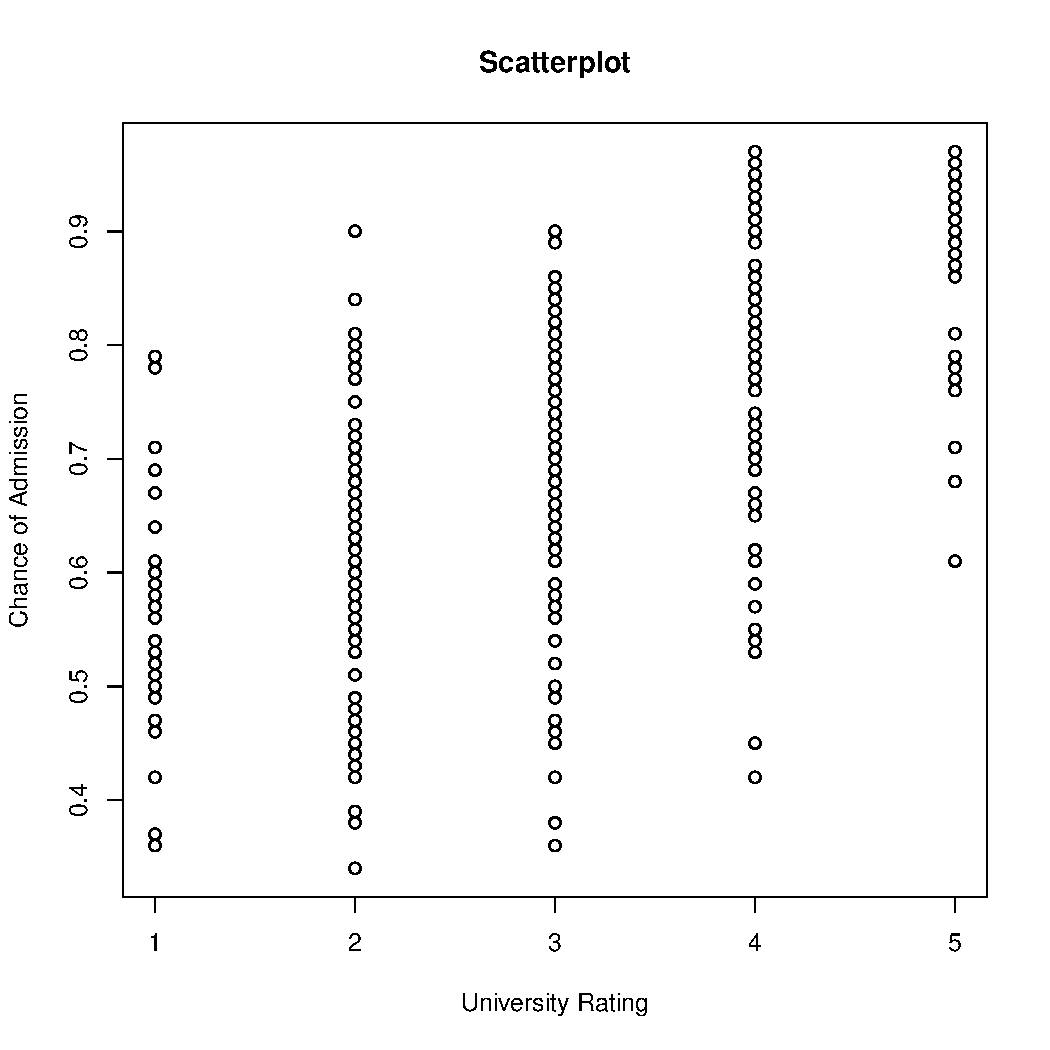
\includegraphics[width=\textwidth]{scatterplotUR.pdf}
            \end{minipage}
        \makebox[\textwidth]{
            \hspace{-10cm} % Adjust the value to align
            \begin{minipage}{0.3\textwidth}
                \centering
                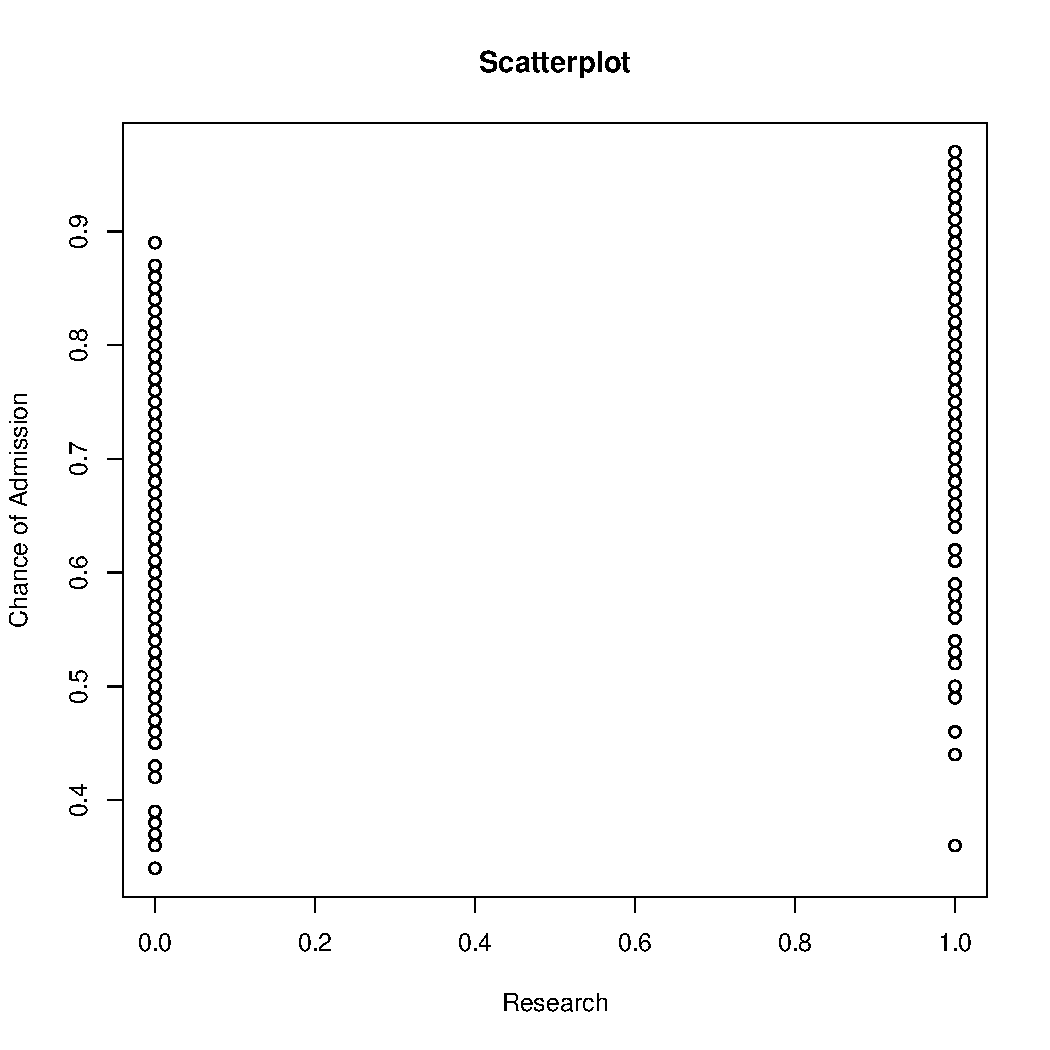
\includegraphics[width=\textwidth]{scatterplotR.pdf}
            \end{minipage}
            }
        \end{figure}
\end{itemize}


\newpage
\subsection{Regression Model}
\label{SW}
\vspace{9pt}
\begin{itemize}
    \item Summary of the Multiple Linear Regression Model 
        \begin{figure} [H]
        \hspace{0.8cm}
            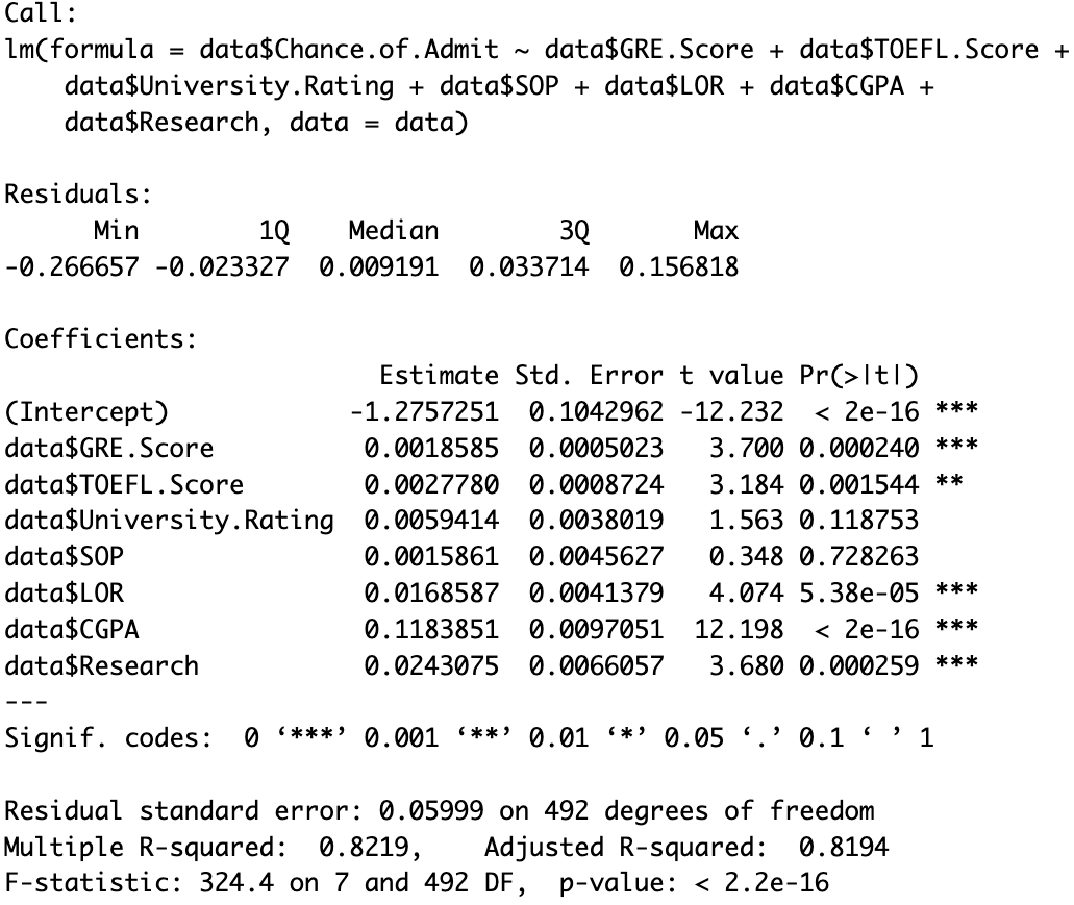
\includegraphics[width=0.8\linewidth]{mregS.pdf}
        \end{figure}
    \item Shapiro-Wilk test for the validity assumptions
        \begin{figure} [H]
        \hspace{0.8cm}
            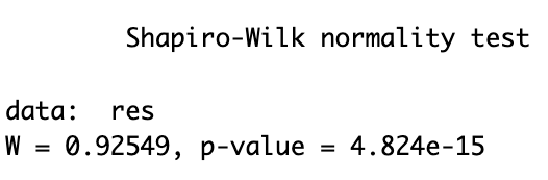
\includegraphics[width=0.4\linewidth]{SW.pdf}
        \end{figure}
    \item Correlation Matrix
        \begin{figure} [H]
        \hspace{0.8cm}
            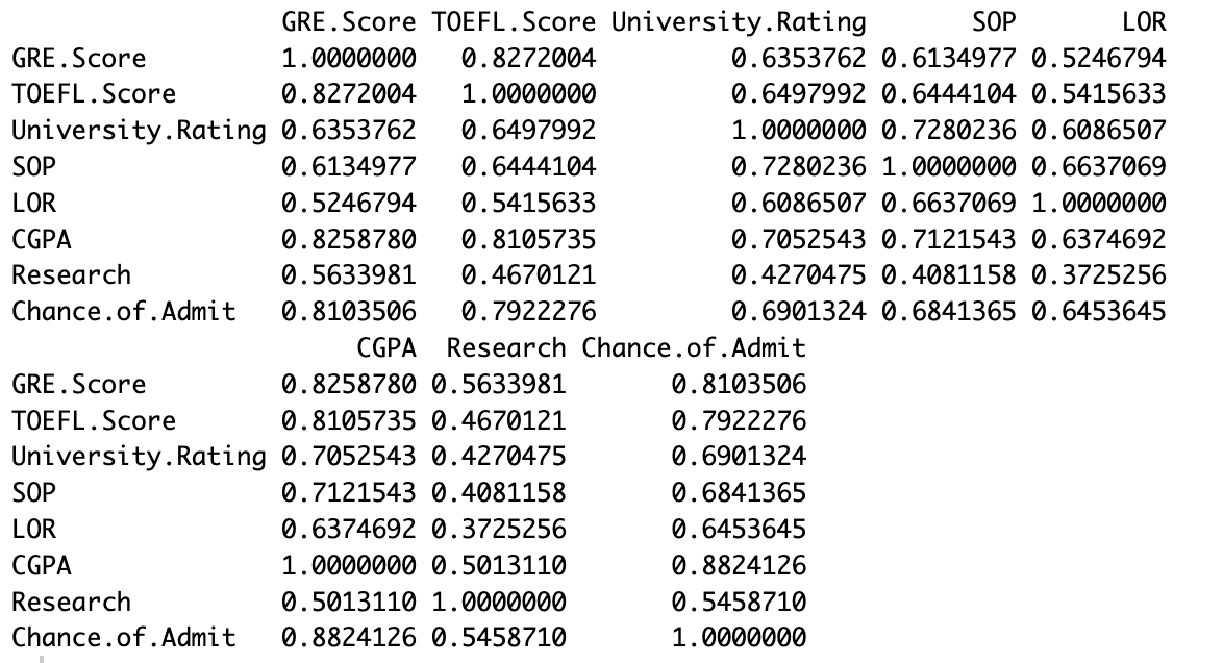
\includegraphics[width=0.8\linewidth]{COR.pdf}
        \end{figure}

    \item Summary of the Interaction Model
        \begin{figure} [H]
        \hspace{0.8cm}
            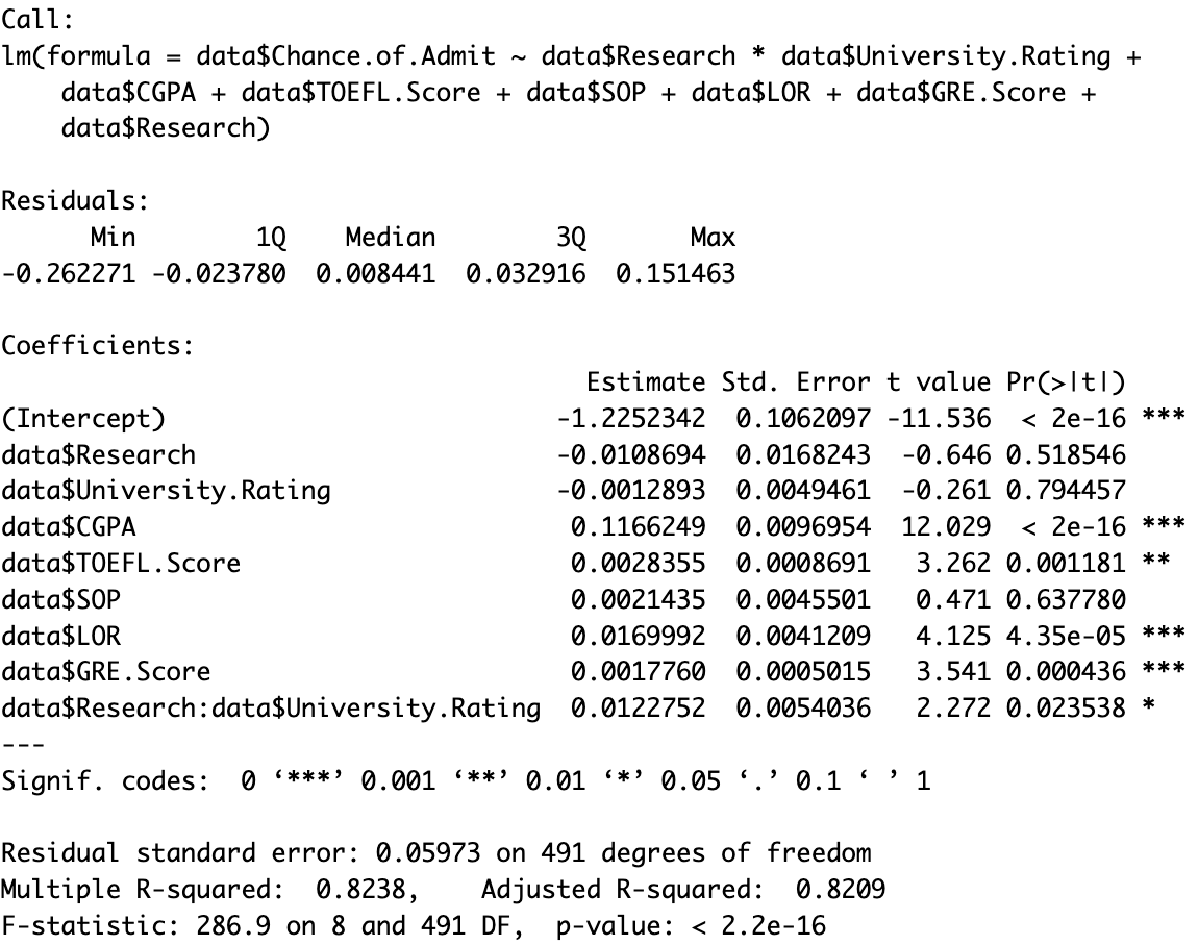
\includegraphics[width=0.8\linewidth]{interaction_modelS.pdf}
        \end{figure}
\end{itemize}


\newpage
\subsection{Model Selection}
\label{MS}
\vspace{10pt}
\begin{itemize}
    \item Step Down Method
        \begin{figure} [H]
            \hspace{0.8cm}
            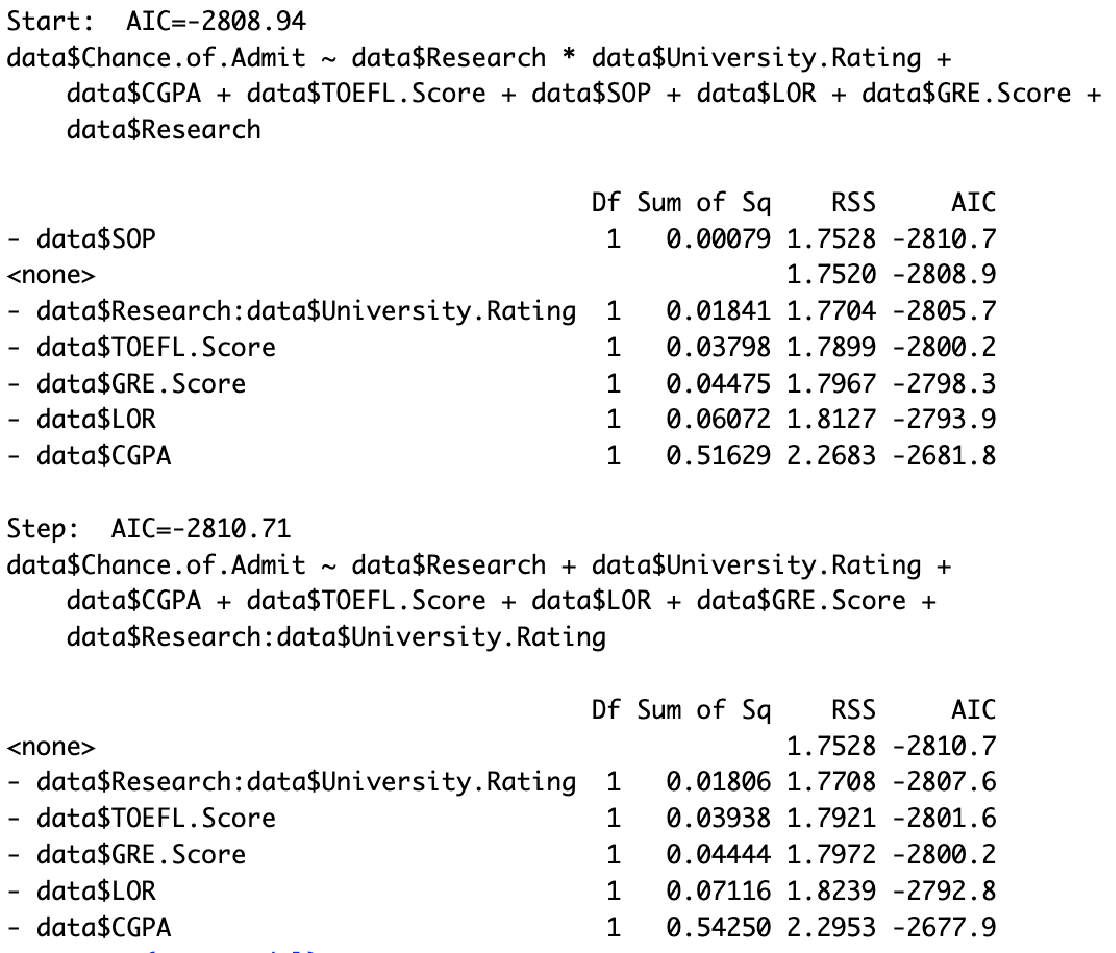
\includegraphics[width=0.8\linewidth]{STEP.pdf}
        \end{figure}
    \item Summary of the Step Model
        \begin{figure} [H]
            \hspace{0.8cm}
            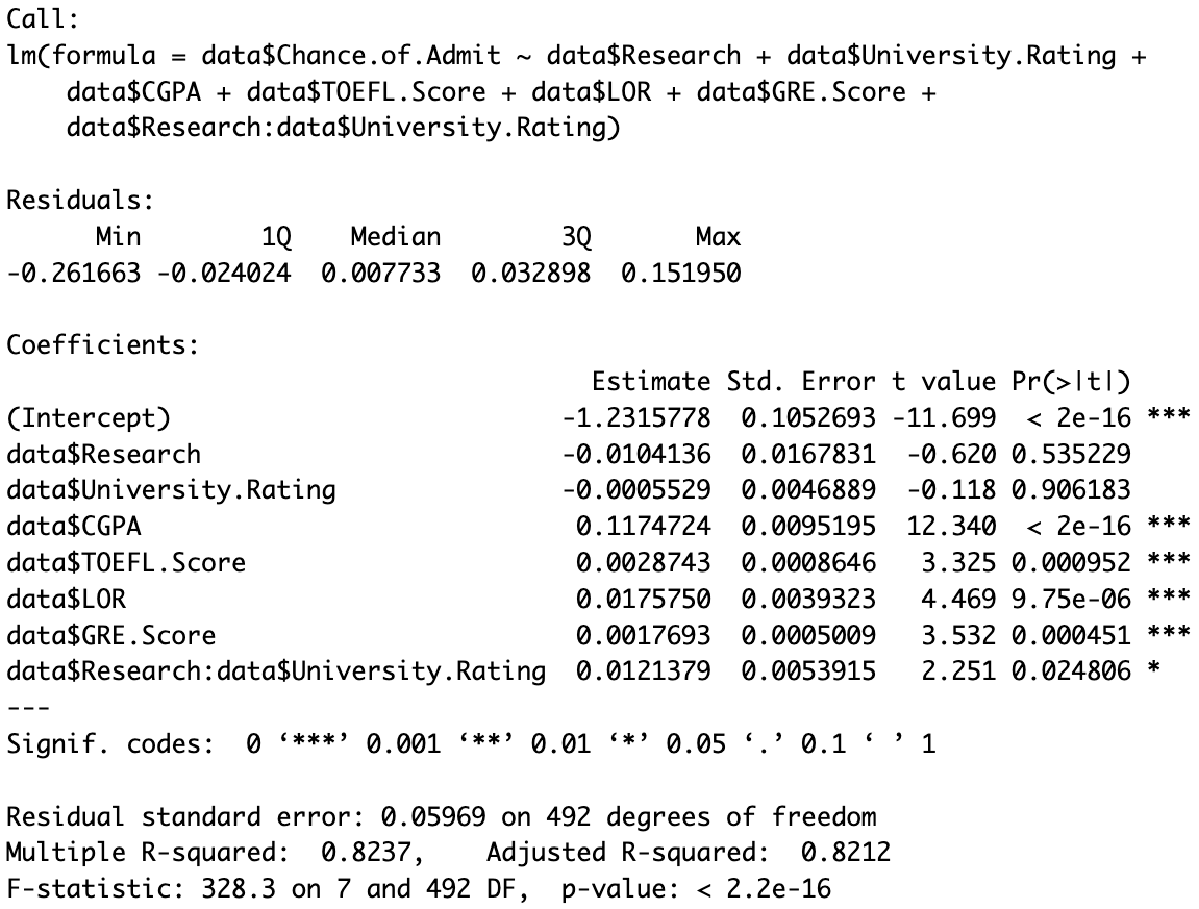
\includegraphics[width=0.8\linewidth]{stepS.pdf}
        \end{figure}
    \item Checking validity assumptions for the Step Model
    \begin{figure}[H]
        \centering
        \begin{minipage}{0.3\textwidth}
            \centering
            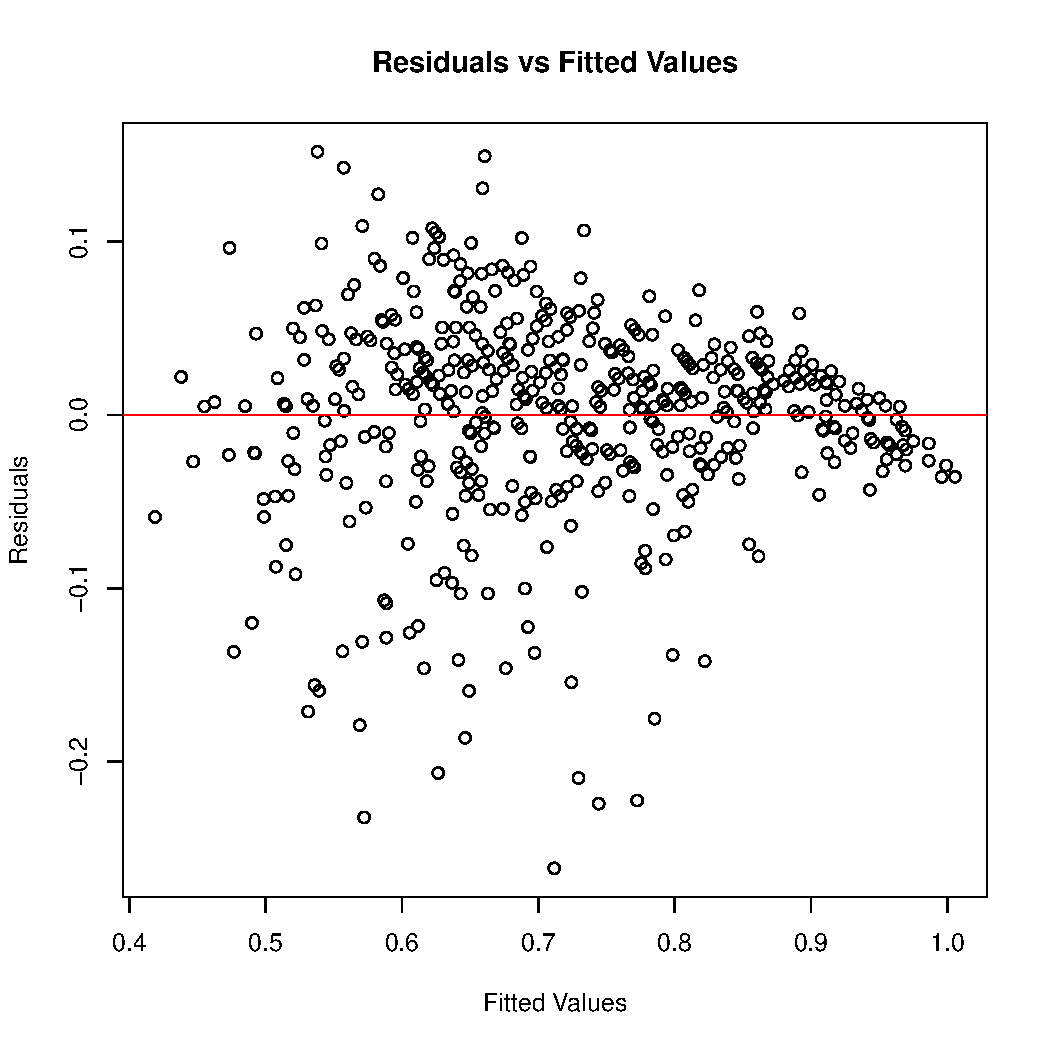
\includegraphics[width=\textwidth]{RFV1.pdf}
        \end{minipage}
        \begin{minipage}{0.3\textwidth}
            \centering
            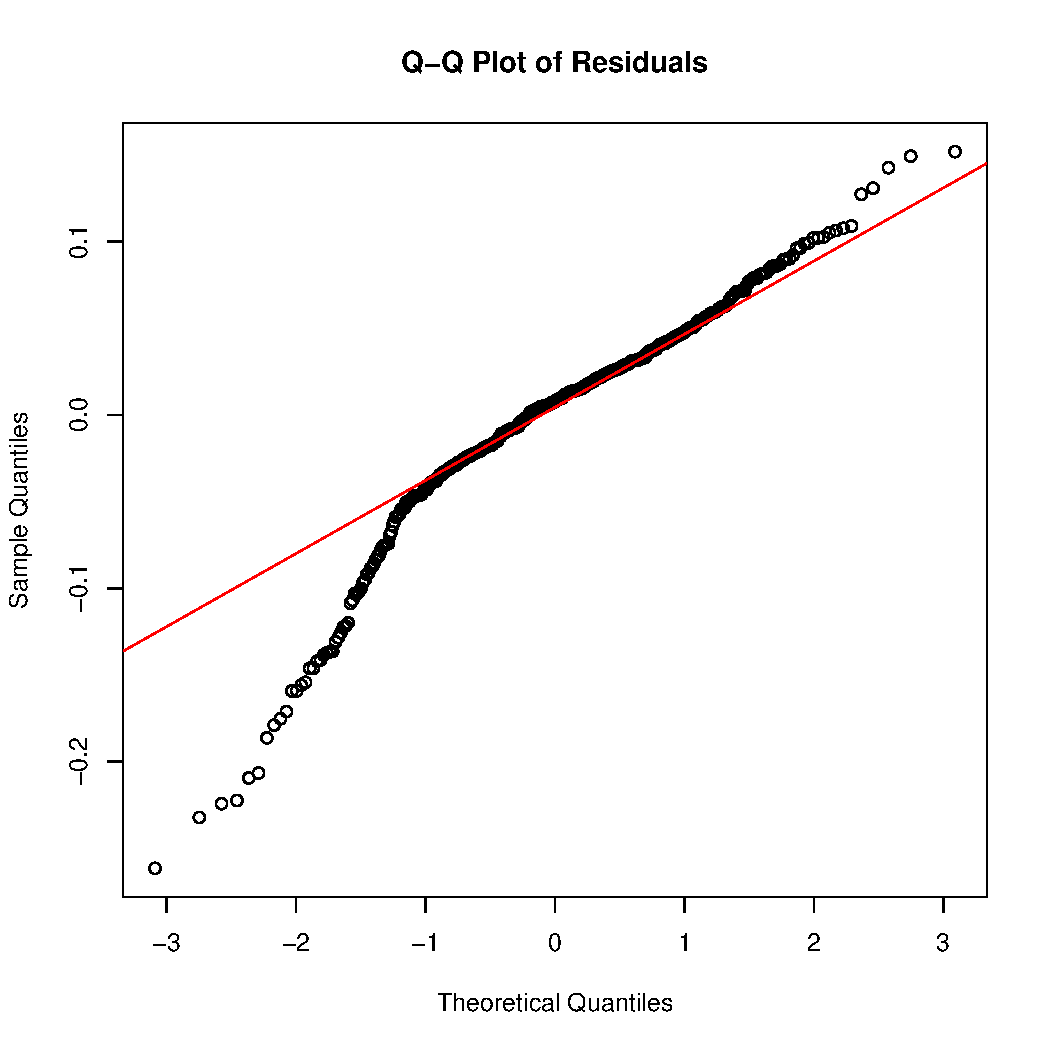
\includegraphics[width=\textwidth]{QQR1.pdf}
        \end{minipage}
        \begin{minipage}{0.3\textwidth}
            \centering
            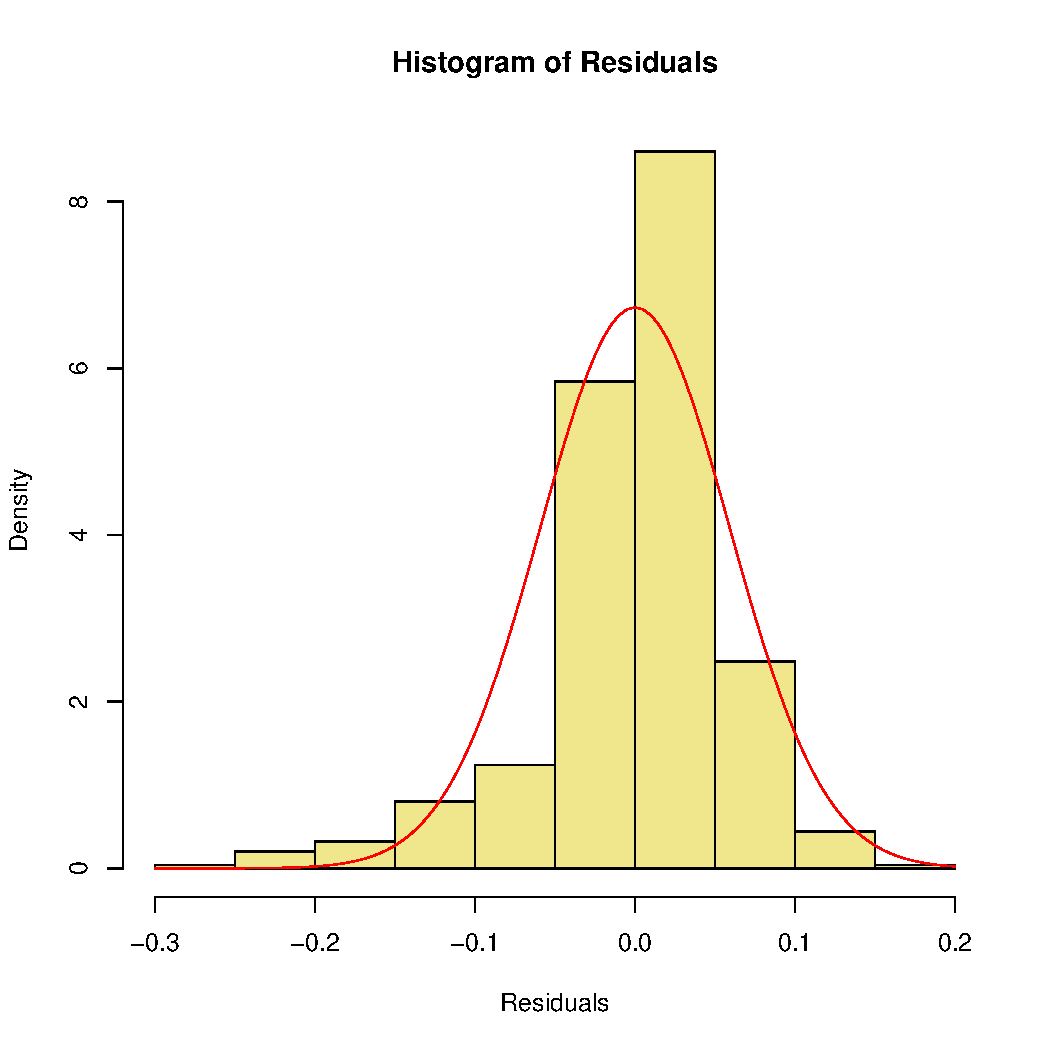
\includegraphics[width=\textwidth]{HR1.pdf}
        \end{minipage}
    \end{figure}
        \begin{figure} [H]
        \hspace{1.2cm}
            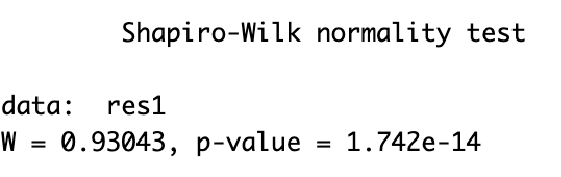
\includegraphics[width=0.4\linewidth]{SW1.pdf}
        \end{figure}
\end{itemize}

\vspace{8cm}
\section{Bibliography}
\label{b}
\begin{itemize}
    \item \href{https://www.kaggle.com/datasets/mohansacharya/graduate-admissions}{Mohan S Acharya, Asfia Armaan, Aneeta S Antony :\textit{A Comparison of Regression Models for Prediction of Graduate Admissions}, IEEE International Conference on Computational Intelligence in Data Science 2019,\textit{Graduate Admission 2}};
    \item Marianne Jonker Fetsje Bijma and Aad van der Vaart. \textit{An Introduction to Mathematical Statistics.} 2nd ed Epsilon Uitgaven, 2016;
    \item 
    \href{https://www.rdocumentation.org/}{R Documentation};    
    \item 
    \href{https://www.statology.org/k-fold-cross-validation-in-r/}
    {Zach Bobbit, \textit{K-Fold Cross Validation in R (Step-by-Step)}};
\end{itemize}
\end{document}
